\documentclass[compress,10pt]{beamer}
% version imprimable pour assistance
%\documentclass[10pt, green, handout]{beamer}
\usepackage[T1]{fontenc}
\usepackage[utf8]{inputenc}
\usepackage[frenchb]{babel} % le document est en français
\usepackage{rotating,amsmath}
\usepackage{graphicx,cancel}       % pour ins\'erer des figures
        % pour d\'efinir plus de couleurs
\usetheme[outer/progressbar=foot]{metropolis}
\setbeamertemplate{section in toc}[sections numbered]
\setbeamertemplate{subsection in toc}[subsections numbered]

%\usetheme{metropolis}  %Applique le theme INRA (ce dernier doit être present dans le repertoire courant)
\usepackage{xcolor,colortbl}
\usepackage{array}
\usepackage{mdframed}
\usepackage{multirow}
\usepackage{lmodern}	
\usepackage{tikz}
\usetikzlibrary{positioning,shapes,arrows}



\setbeamerfont{bibliography item}{size=\tiny}
\setbeamerfont{bibliography entry author}{size=\tiny}
\setbeamerfont{bibliography entry title}{size=\tiny}
\setbeamerfont{bibliography entry location}{size=\tiny}
\setbeamerfont{bibliography entry note}{size=\tiny}
            

\definecolor{dgreen2}{RGB}{102,193,191}
%RGB()
\definecolor{dgreen}{RGB}{255,165,0}
\definecolor{mygrey}{RGB}{230,230,230}


\setbeamertemplate{blocks}[rounded][shadow=true]
\setbeamercolor{block title}{use = structure  ,bg=mygrey, fg=dgreen}
%\setbeamercolor{normal text}{fg=black,bg=white}
%\setbeamercolor{alerted text}{fg=lgreen}
%\setbeamercolor{example text}{fg=lgreen}
%\setbeamercolor{structure}{fg=dgreen} %d'où ce bleu par défaut
\setbeamercolor{background canvas}{parent=normal text}


\usepackage{tikz}
\usetikzlibrary{calc,shapes,backgrounds,arrows,automata,shadows,positioning}
\setbeamertemplate{frametitlecontinuation}{\insertcontinuationcountroman}

%-------------------------------------------------------------------------------
% Quelques options pdf
%-------------------------------------------------------------------------------
\hypersetup{
pdfpagemode = FullScreen, % afficher le pdf en plein \'ecran
pdfauthor   = {},%
pdftitle    = {},%
pdfsubject  = {},%
pdfkeywords = {Science,Impact},%
pdfcreator  = {PDFLaTeX,emacs,AucTeX},%
pdfproducer = {INRAE}%
}


\newcommand\Wider[2][3em]{%
\makebox[\linewidth][c]{%
  \begin{minipage}{\dimexpr\textwidth+#1\relax}
  \raggedright#2
  \end{minipage}%
  }%
}

\AtBeginSection[]
{  \begin{frame}
  \frametitle{}
  \tableofcontents[currentsection, hideothersubsections]
  \end{frame} 
}
%  \AtBeginSubsection[]
%  {  \begin{frame}
%    \frametitle{}
%    \tableofcontents[currentsubsection, currentsection,hideothersubsections, subsectionstyle=show/shaded/hide]
%    \end{frame} 
%  }






%
\usepackage{amsmath}

% TikZ
\newcommand{\nodesize}{2em}
\newcommand{\edgeunit}{2.5*\nodesize}
\tikzstyle{hidden}=[draw, circle, fill=gray!50, minimum width=\nodesize, inner sep=0]
\tikzstyle{observed}=[draw, circle, minimum width=\nodesize, inner sep=0]
\tikzstyle{not observed}=[draw, circle, minimum width=\nodesize, color=gray!20, inner sep=0]

\tikzstyle{eliminated}=[draw, circle, minimum width=\nodesize, color=gray!50, inner sep=0]
\tikzstyle{empty}=[]
\tikzstyle{arrow}=[->, >=latex, line width=1pt]
\tikzstyle{edge}=[-, line width=1pt]
\tikzstyle{dashedarrow}=[->, >=latex, dashed, line width=1pt]
\tikzstyle{lightarrow}=[->, >=latex, line width=1pt, fill=gray!50, color=gray!50]

% %#################################"
% 
% \usepackage{amsmath}
% \DeclareMathOperator*{\argmax}{arg\,max}
% \DeclareMathOperator*{\argmin}{arg\,min}
% \newcommand{\bX}{\boldsymbol{Y}}
% \newcommand{\pr}{\mathbb{P}}
% \newcommand{\E}{\mathbb{E}}
% 
% \newcommand{\Xall}{\bX}
% 
% \newcommand{\Zall}{\bZ}
% \newcommand{\M}{\mathcal{M}_{Q}}
% \newcommand{\ind}{\mathds{1}}
% \newcommand{\Mcal}{\mathcal{M}}
% \newcommand{\Qcal}{\mathcal{Q}}
% \newcommand{\colSBM}{colSBM}
% 
% \newcommand{\bZ}{\boldsymbol{Z}}
% \newcommand{\bpi}{\boldsymbol{\pi}}
% \newcommand{\balpha}{\boldsymbol{\alpha}}
% \newcommand{\btau}{\boldsymbol{\tau}}
% 
% 
% \def\Ecal{\mathcal{E}}
% 
% 
% 
% \def\N{\mathbb{N}}
% \def\R{\mathbb{R}}
% \def\F{\mathcal{F}}
% \def\Nb{\boldsymbol{N}}
% \def\bZ{\boldsymbol{Z}}
% \def\btheta{\boldsymbol{\theta}}
% \def\bpi{\boldsymbol{\pi}}
% \def\bY{\boldsymbol{Y}}
% \def \ind{\mathbb{I}}
% \def \P{\mathbb{P}}
% \def \pen{\mbox{Pen}}
% \def \SBM{\mbox{SBM}}
% 
% \newcommand{\lat}{\mathbf{Z}}
% \newcommand{\Xm}{Y^{m}}
% \newcommand{\Zm}{Z^{m}}
% \newcommand{\pim}{\pi^{m}}
% \newcommand{\alpham}{\alpha^{m}}
% \newcommand{\taum}{\tau^{m}}
% \newcommand{\con}{\alpha}
% \newcommand{\conm}{\alpha^{m}}
% \newcommand{\dens}{\delta}
% \newcommand{\nm}{n_m}

%\newcommand{\myemph}[1]{\textbf{\textcolor{dgreen}{#1}}}


\def\N{\mathbb{N}}
\def\R{\mathbb{R}}
\def\F{\mathcal{F}}
\def\Nb{\boldsymbol{N}}

\def \vert{\color{dgreen}}
\def \noir{\color{black}}
\def \rouge{\color{red}}

\def \SBM{\mbox{SBM}}


\newcommand{\indep}{\perp \!\!\! \perp}

\newcommand{\Ibb}{\mathbf{1}}
\newcommand{\E}{\mathbb{E}}
\newcommand{\Esp}{\mathbb{E}}
\newcommand{\Var}{\mathbb{V}}
\newcommand{\KL}{\mbox{KL}}
\renewcommand{\P}{\mathbb{P}}

\DeclareMathOperator*{\argmax}{arg\,max}
\DeclareMathOperator*{\argmin}{arg\,min}
\newcommand{\ICL}{\mathrm{ICL}}
\newcommand{\BIC}{\mathrm{BIC}}
\newcommand{\MC}{\mathrm{MC}}
\newcommand{\pen}{\mathrm{pen}}
\newcommand{\ind}{\mathbf{1}}


\newcommand{\diag}{\mathop{\mathrm{diag}}}
\newcommand{\bbeta}{\boldsymbol{\beta}}
\newcommand{\balpha}{\boldsymbol{\alpha}}
\newcommand{\btheta}{\boldsymbol{\theta}}
\newcommand{\bY}{\mathbf{Y}}
\newcommand{\obs}{\mathbf{Y}}
\newcommand{\Xm}{\mathbf{Y}^m} 
\newcommand{\M}{\mathcal{M}_{\bK}}
\newcommand{\balpham}{\balpha^{m}}
\newcommand{\bpim}{\bpi^{m}}
\newcommand{\deltam}{\delta_{m}}
\newcommand{\Sc}{\text{Sc}}
\newcommand{\Mcal}{\mathcal{M}}
\newcommand{\Ncal}{\mathcal{N}}
\newcommand{\Fcal}{\mathcal{F}}
\newcommand{\Pcal}{\mathcal{P}}
\newcommand{\Rcal}{\mathcal{R}}
\newcommand{\Gcal}{\mathcal{G}}
\newcommand{\Qcal}{\mathcal{Q}}
\newcommand{\bK}{\mathbf{K}}
\newcommand{\bX}{\mathbf{Y}}
\newcommand{\Xall}{\mathbf{Y}}
\newcommand{\Zall}{\mathbf{Z}}
\newcommand{\bpi}{\boldsymbol{\pi}}
\newcommand{\btau}{\mathbf{\tau}}
\newcommand{\bZ}{\mathbf{Z}}
\newcommand{\by}{\mathbf{y}}
\newcommand{\ba}{\mathbf{a}}
\newcommand{\bt}{\mathbf{t}}
\newcommand{\bx}{\mathbf{x}}
\newcommand{\bz}{\mathbf{z}}
\newcommand{\bh}{\mathbf{h}}
\newcommand{\bc}{\mathbf{c}}
\newcommand{\bb}{\mathbf{b}}
\newcommand{\bB}{\mathbf{B}}
\newcommand{\bC}{\mathbf{C}}
\newcommand{\bM}{\mathbf{M}}
\newcommand{\bphi}{\boldsymbol{\phi}}
\newcommand{\blambda}{\boldsymbol{\lambda}}
\newcommand{\bepsilon}{\boldsymbol{\epsilon}}
\newcommand{\bgamma}{\boldsymbol{\gamma}}
\newcommand{\bpsi}{\boldsymbol{\psi}}
\newcommand{\bm}{\mathbf{m}}
\newcommand{\dd}{\;\text{d}}
\newcommand{\Hcal}{\mathcal{H}}
\newcommand{\Prob}{\text{P}}
\newcommand\Ccancel[2][black]{\renewcommand\CancelColor{\color{#1}}\cancel{#2}}

\newcommand{\Zm}{Z^{m}}
\newcommand{\pim}{\pi^{m}}
\newcommand{\alpham}{\alpha^{m}}
\newcommand{\con}{\alpha}
\newcommand{\conm}{\alpha^{m}}
\newcommand{\dens}{\delta}
\newcommand{\nm}{n_m}
\newcommand{\colSBM}{colSBM}


\newcommand{\BICL}{\text{BIC-L}}
\newcommand{\eBICL}{\text{eBIC-L}}
\newcommand{\iidcolSBM}{iid\text{-}\colSBM}
\newcommand{\denscolSBM}{\dens\text{-}\colSBM}
\newcommand{\picolSBM}{\pi\text{-}\colSBM}
\newcommand{\denspicolSBM}{\dens\pi\text{-}\colSBM}
\newcommand{\sepSBM}{sep\text{-}SBM}





\title{Stochastic block models for  a collection  of networks}
\subtitle{Applications in ecology and sociology}
\date{}
\author{Sophie  Donnet,  
\includegraphics[width= 1cm]{plots/Logo-INRAE},    MIA Paris-Saclay 
\includegraphics[width= 0.5cm]{plots/MIAPS}}
\institute{Aug. 2023}
\titlegraphic{\hfill
\includegraphics[width= 0.3  \textwidth]{plots/Logo-INRAE}}



\begin{document}

\maketitle



%----------------------------------------------------
\begin{frame}{Collaborators}
%----------------------------------------------------
 Joint work with 
 
\begin{center}
\begin{tabular}{ccc}

\includegraphics[width = 0.25\linewidth]{plots/Barbillon}& 
\includegraphics[width = 0.25\linewidth]{plots/saintclair} \\
 \scriptsize P. Barbillon & \scriptsize S.C. Chabert-Liddell\\
 \scriptsize (AgroParisTech) & \scriptsize (INRAE) 
\end{tabular}
\end{center}

 
\end{frame}

%----------------------------------------------------
\begin{frame}{Collection of networks: consensus in the structure}
%----------------------------------------------------
\begin{block}{Objectives}
Looking for  commun patterns in networks involving non-common sets of nodes
\end{block}
\begin{center}
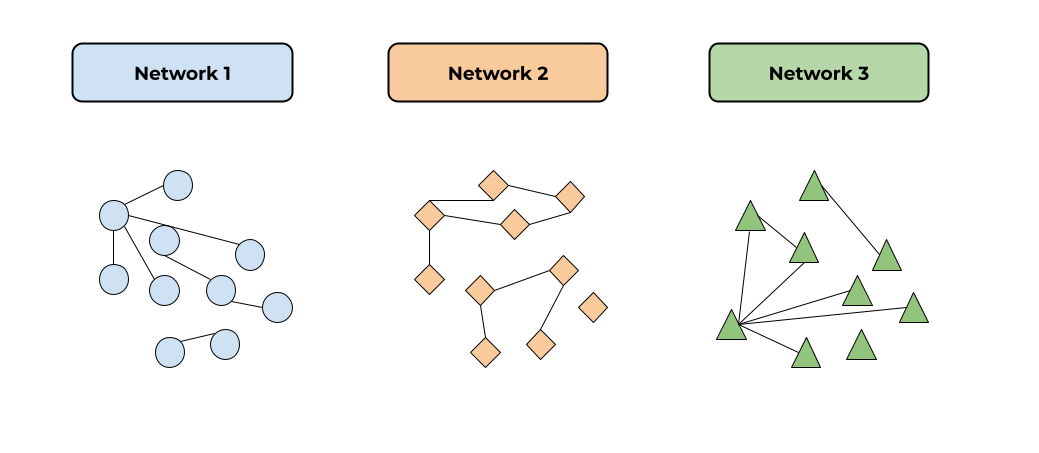
\includegraphics[width = 0.7\linewidth]{plots/ConsensusNetwork}
\end{center}
\textbf{Applications}
\begin{itemize}
 \item Compare the structure of ecological networks
 \item Compare sociological networks : advices between lawyers, researchers  or priests
\end{itemize}

\end{frame}




%====================================================================
\begin{frame}{Three foodwebs }
%====================================================================
\begin{itemize}
\item Pine-firest stream food webs issued from Maine, North-Caroline and Nez-Zealand  {\footnotesize \color{dgreen} \cite{thompson2003impacts}}
\item Involve respectively $105$, $58$ and  $71$ species.
\item $Y_{ij}=1$ if $i$ is eaten by $j$.  Directed relation
\begin{center}
    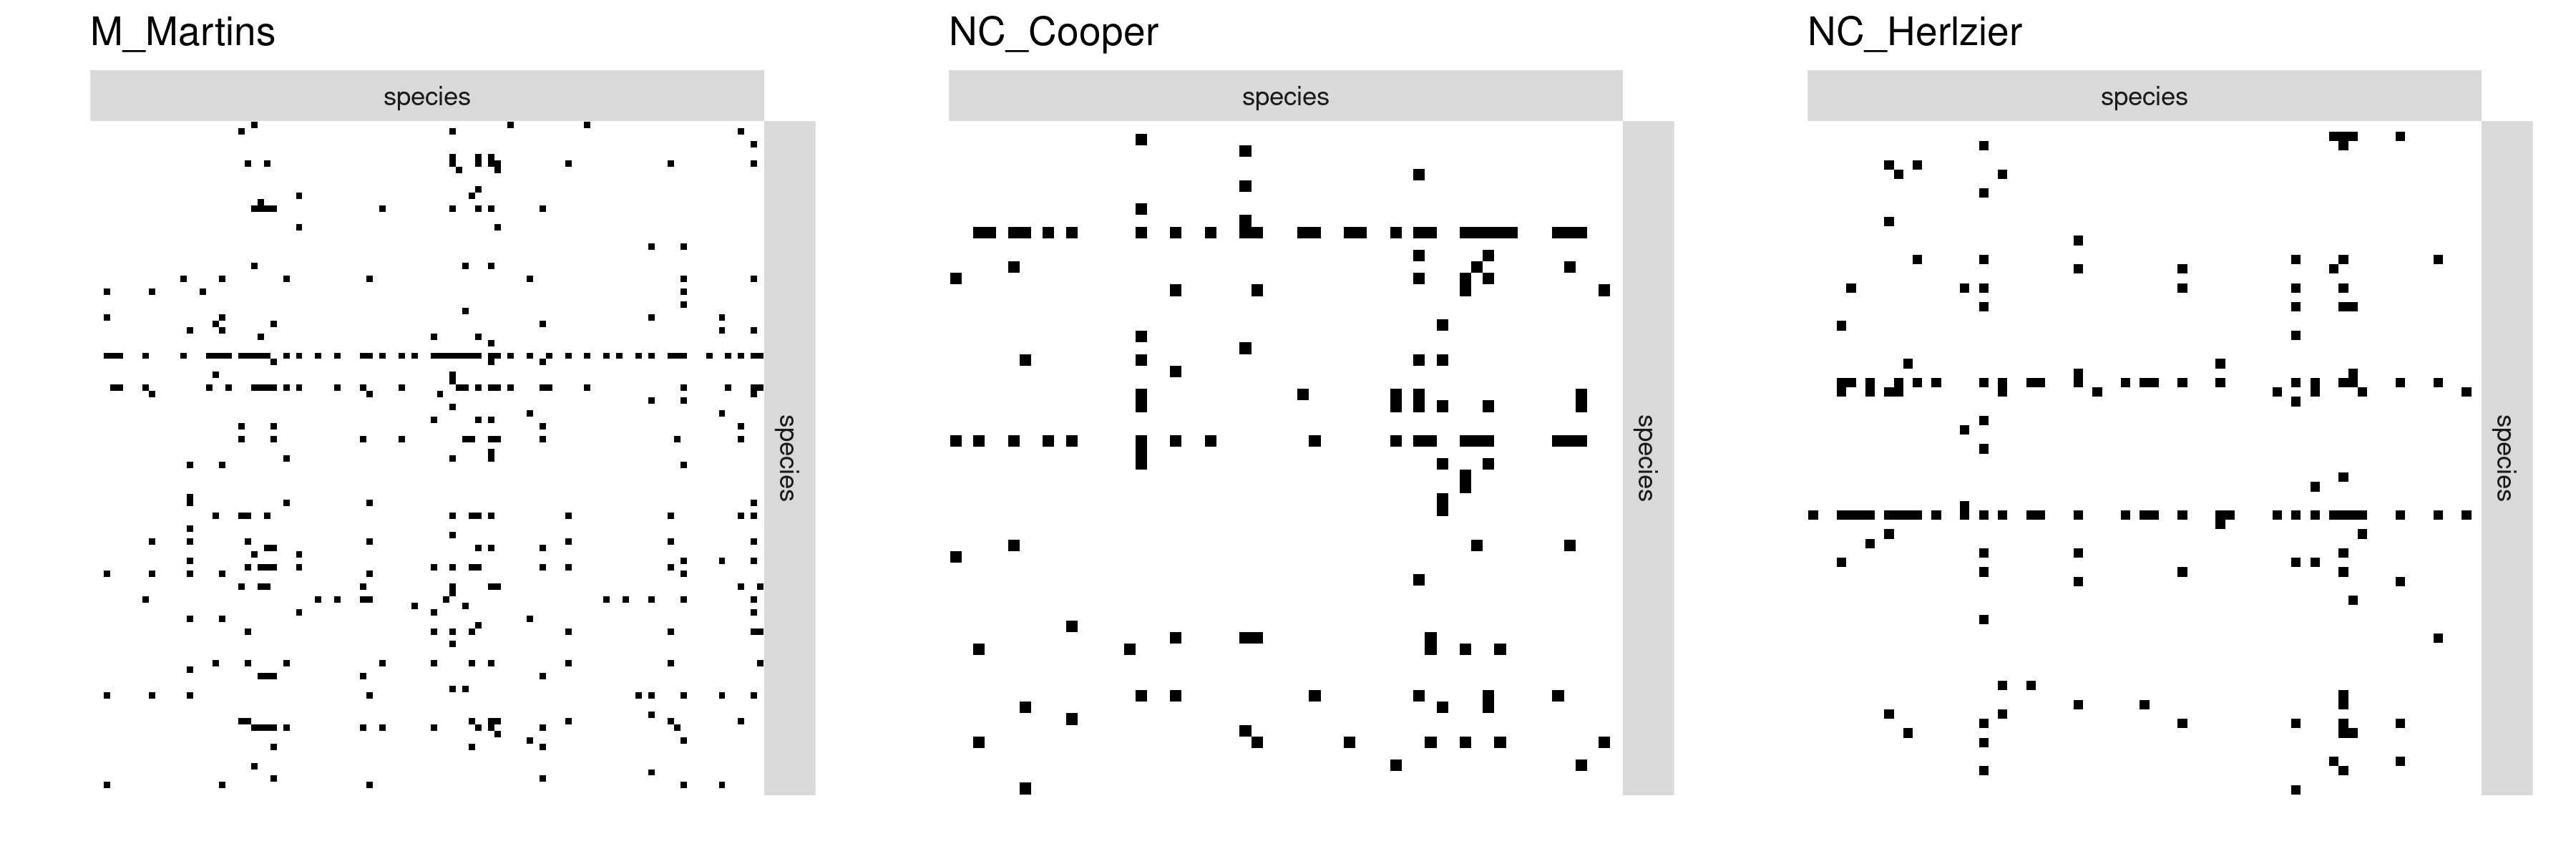
\includegraphics[width = \textwidth]{plots/rawdata}
\end{center}

\item Look for similarities and differences between network structures. 
\end{itemize}
\end{frame}

%====================================================================
\begin{frame}{Separate  SBMs}
%==================================================================


 \centering{
    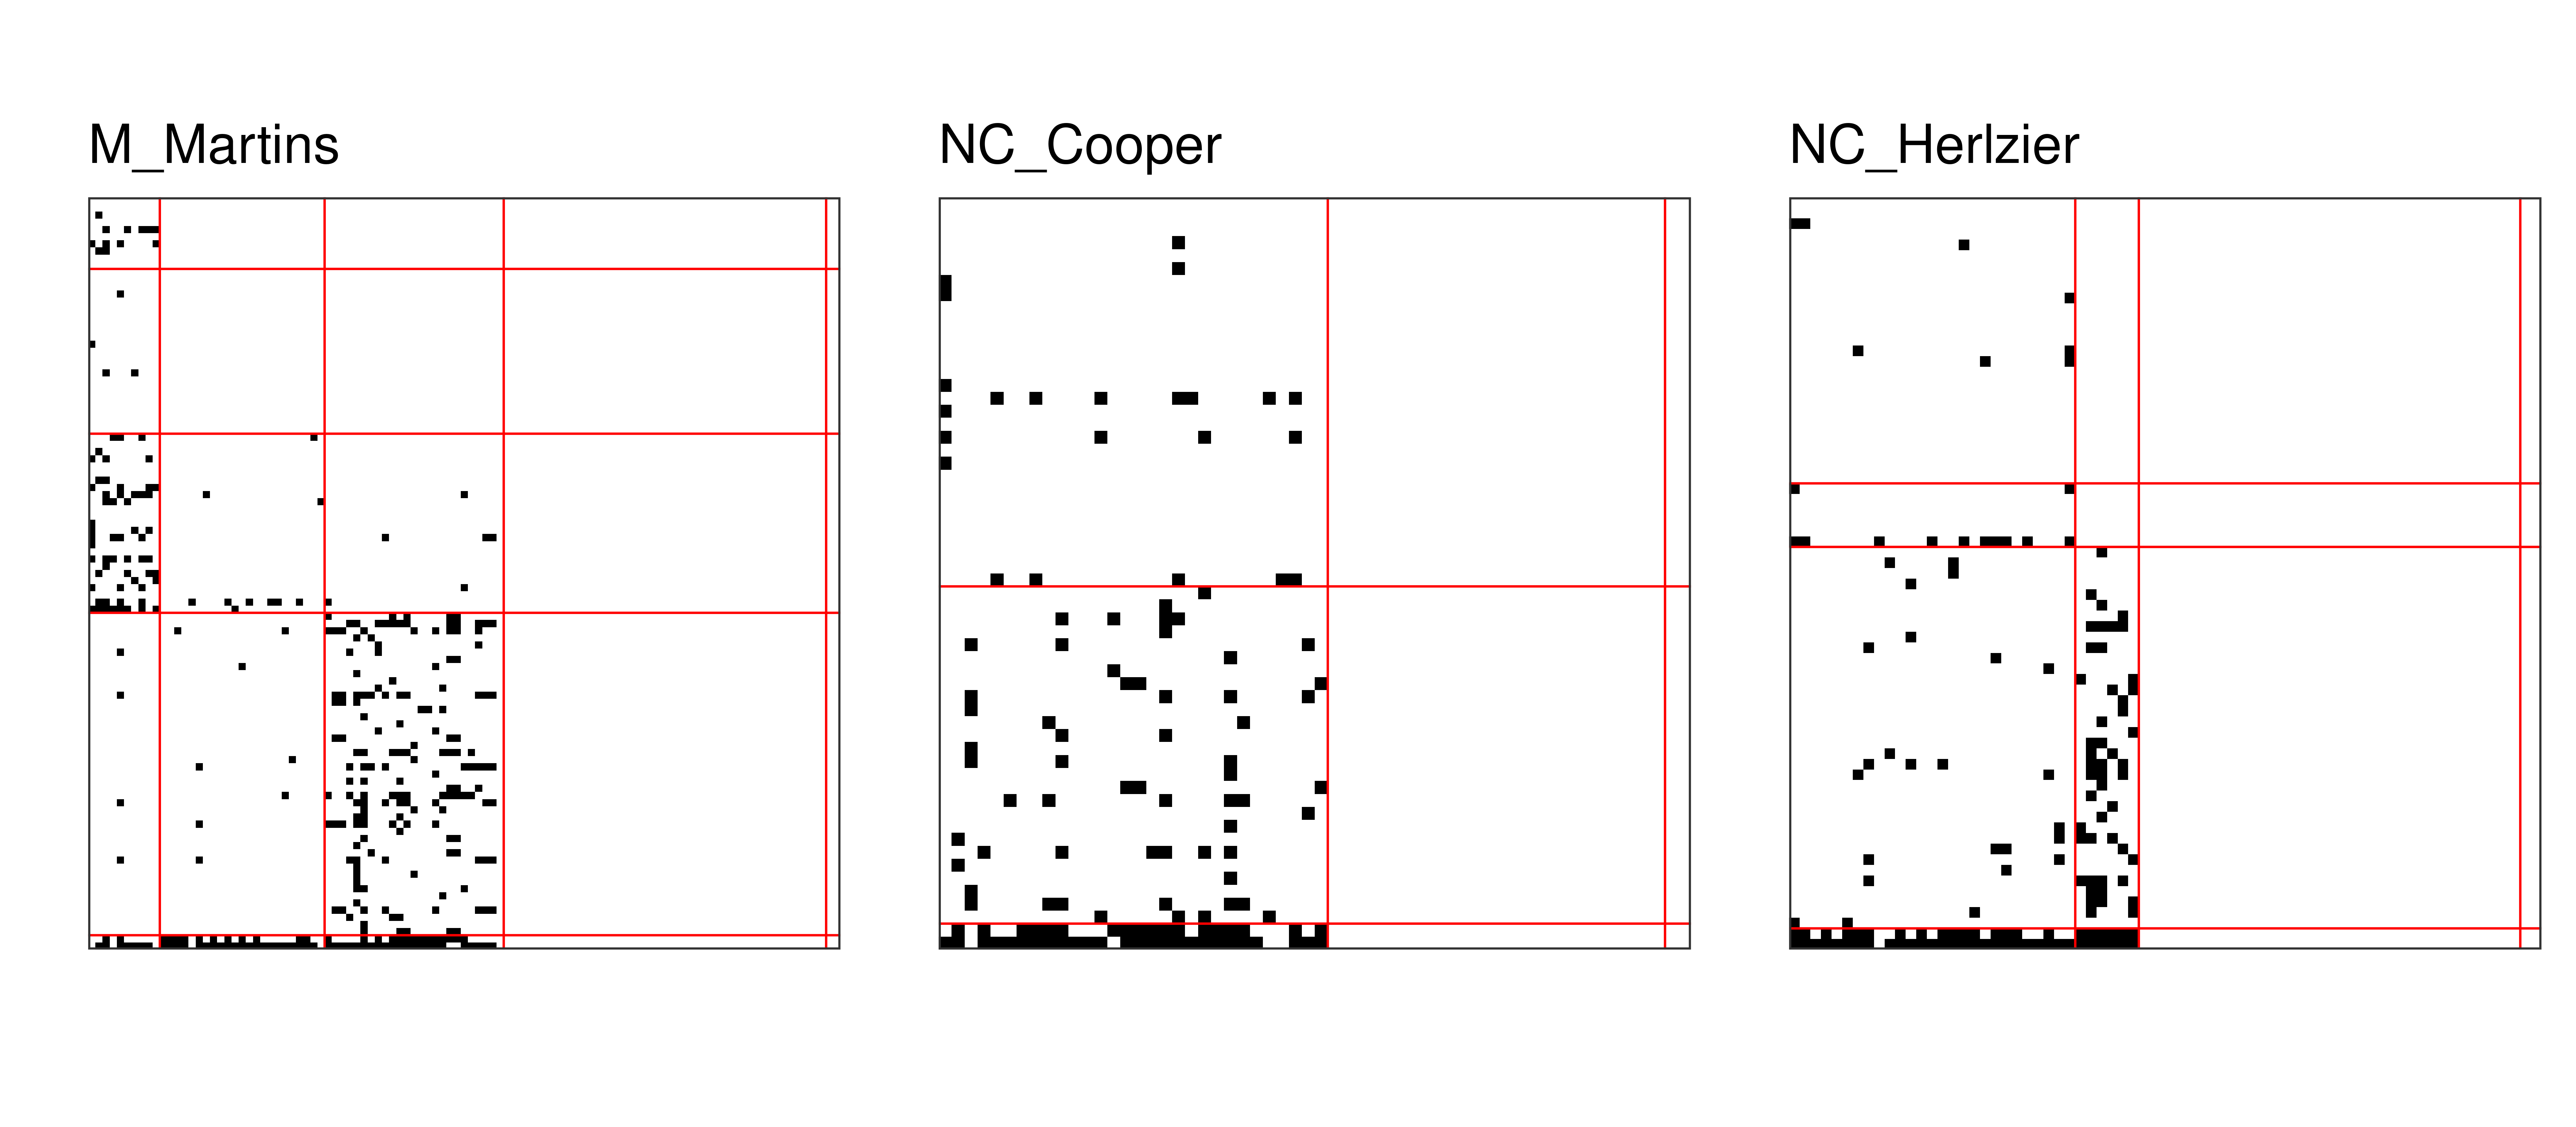
\includegraphics[width = .8\textwidth]{plots/plot_sbm_3net}}
   
   
 \begin{itemize}
  \item Fitted SBM on each separately
  \item Reordered the matrices following the blocks
   \item Label the blocks following the  average out-degrees order
   \end{itemize}

   
Interpretation:
  \begin{itemize}
   \item In row : is eaten by... 
   \item In col : eats... 
  \end{itemize}
  
\end{frame}

%====================================================================
\begin{frame}{Separate  SBMs}
%==================================================================
 \centering{
    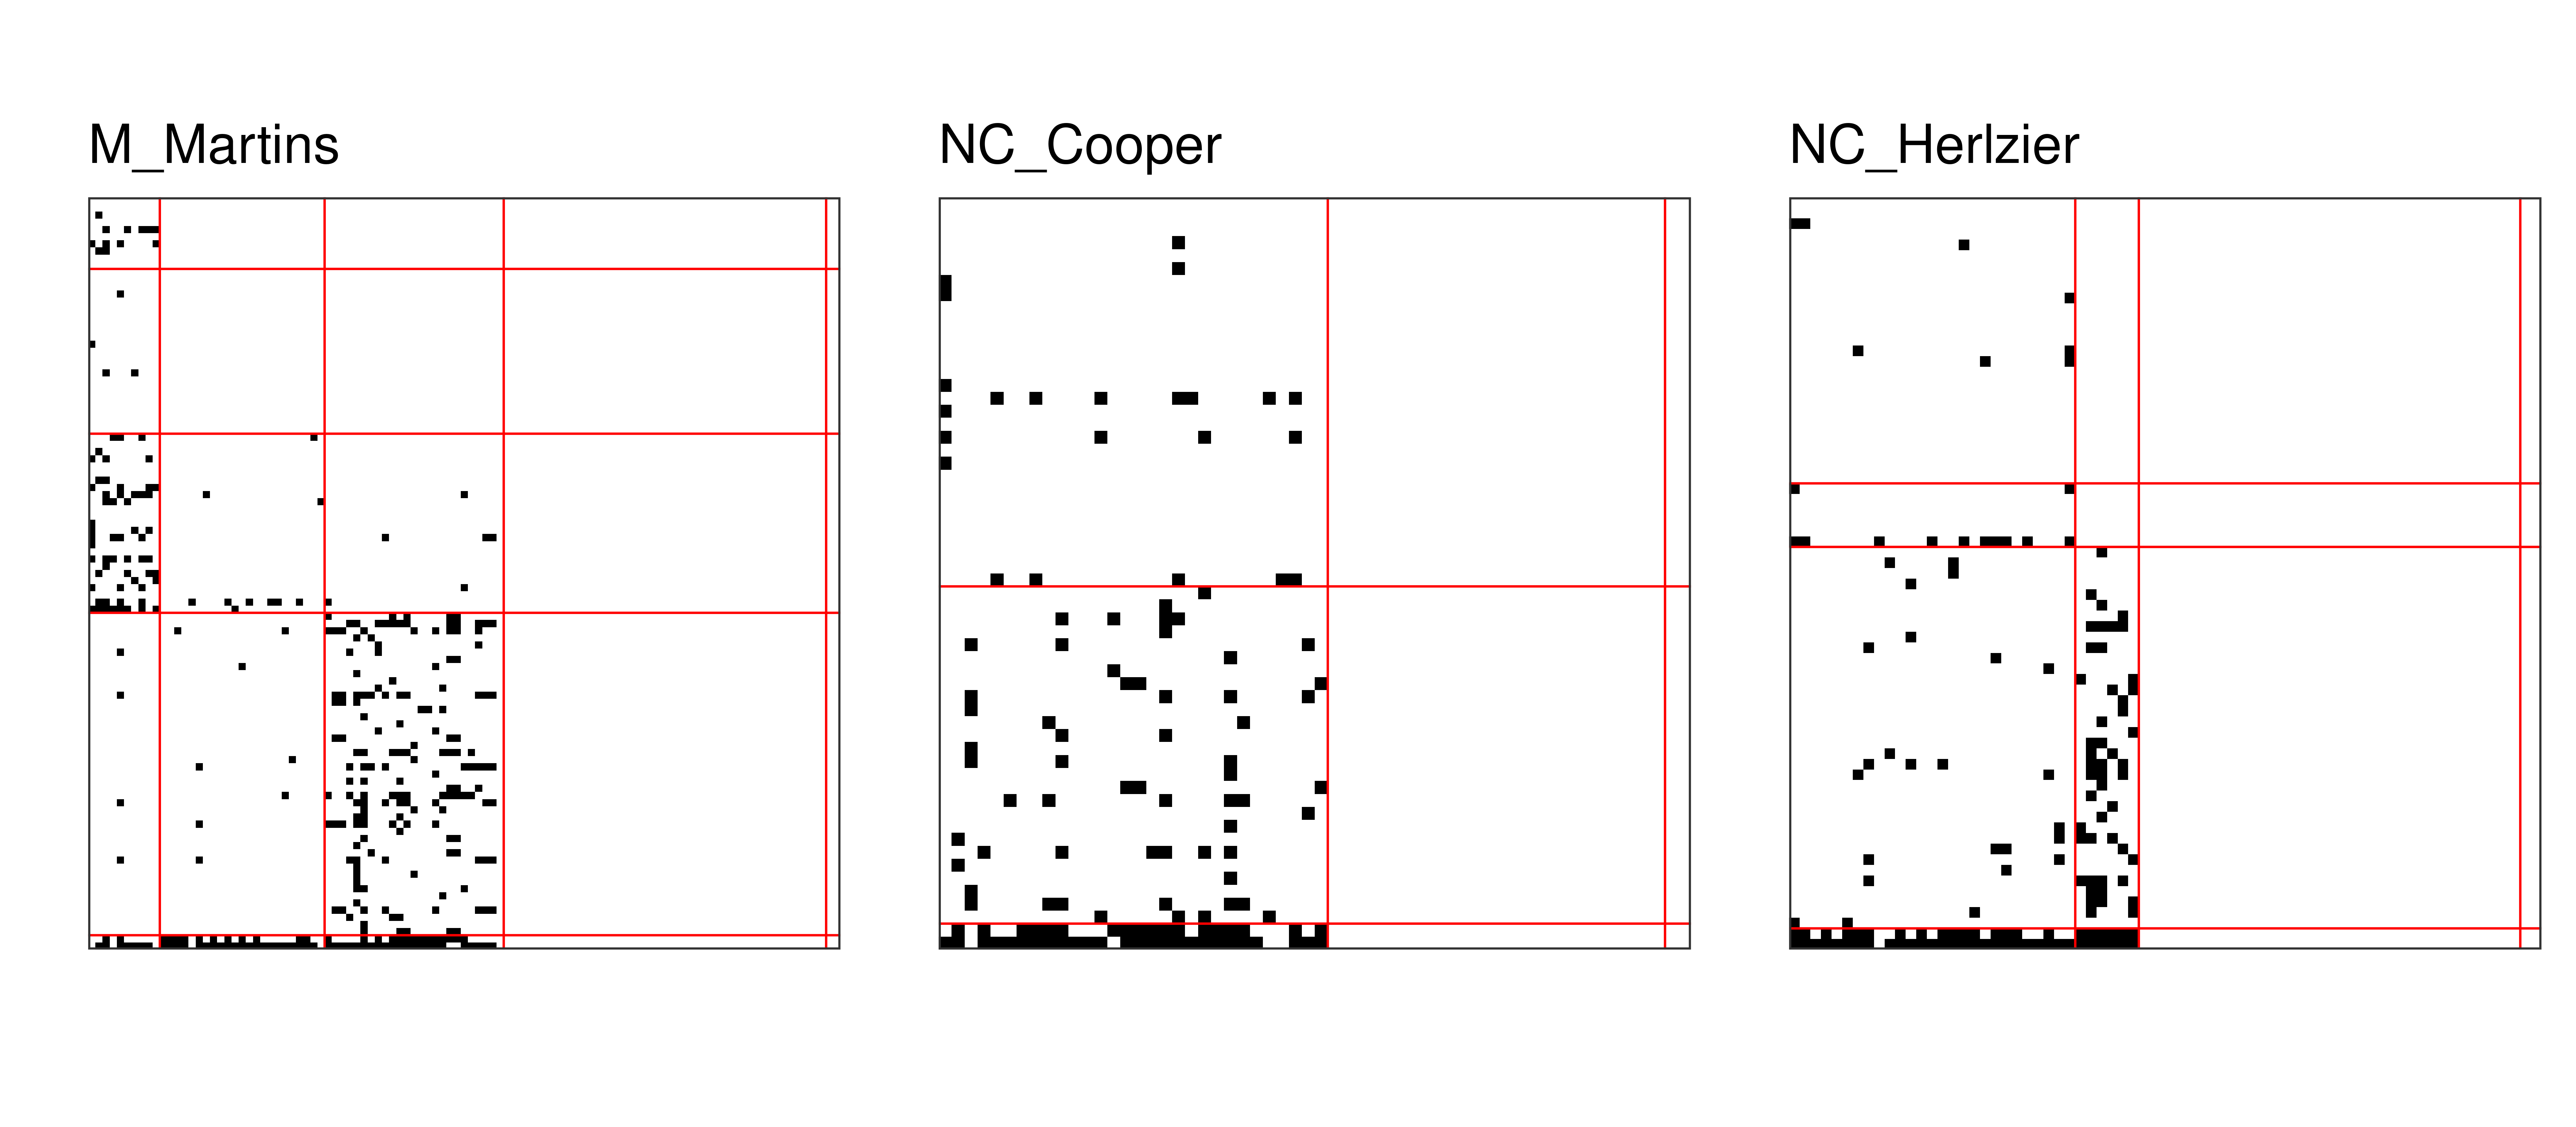
\includegraphics[width = .8\textwidth]{plots/plot_sbm_3net}}
   
   
   
 \begin{itemize}
  \item Two bottom groups in each matrix are basal species : 
  eaten by many species and not eating anybody. 
  \item 
  \begin{itemize}
  \item \textbf{Martins}:  has a separation into $5$ blocks, the third one is a medium trophic level, which preys on basal species and is highly preyed by species of the $1$st block.
 \item 
  \textbf{Cooper}. Higher trophic levels grouped together in the same block (lack of statistical power). 
  \item \textbf{Herlzier}:  higher trophic level is separated into $2$ blocks determined on how much they prey on the less preyed basal block. 
  
\end{itemize}
\end{itemize}
   
\end{frame}






 



%==================================================================
\begin{frame}{Towards a joint modeling of the networks}
%==================================================================
 
 
 \begin{itemize}
  \item Need to model jointly the networks
  \item Identify the groups playing the same role through out the networks, with an unsupervised strategy.  
 \end{itemize}
 
 
\begin{block}{A joint model}
 Let $(\bY^m)_{m=1,\dots,M}$ denote the collection of networks each involving $n_m$ nodes. 
 \begin{itemize}
  \item Set $$\bY^m \sim_{ind} \SBM_{n_m}(Q^m, \bpi^m, \balpha^m)$$
  \item Design conditions on the parameters $(\bpi^m)_{m=1,\dots,M}$ and $(\balpha^m)_{m=1,\dots,M}$
 \end{itemize}
\end{block}

 \end{frame}
 



\subsection{A SBM for a collection of networks}
 
%======================================================
\begin{frame}{First model}
%=======================================================

\begin{block}{iid-colSBM}
 \begin{equation*}\label{mod:iid}
\bY^m \sim \SBM_{n_m}(Q,\bpi, \balpha)
\end{equation*}
with $\pi_{q} >0 $ $\forall q  \in  \{1,\dots, Q\}$ and $\sum_{q  = 1}^Q \pi_{q} = 1$.
\end{block}
\begin{itemize}
\item  $(Q-1)+Q^2$ unknown parameters, $M$ clustering $Z^{m}$
\item  Too strict to be applied to the Thomson's dataset? 
\end{itemize}


\end{frame}





%======================================================
\begin{frame}{A first relaxed model : $\pi$-colSBM}
%=======================================================

Same structure of connection  $\alpha$, specific proportions of blocks in each network
 
 
\begin{block}{$\pi$-colSBM}
 \begin{equation*}\label{mod:iid}
\bY^m \sim \SBM_{n_m}(Q, \bpi^m, \balpha)
\end{equation*}
 
\end{block}

\textbf{On the block proportions}
\begin{itemize}
\item  $\pim_q \geq 0$
\item If $\pim_q=0$ then  block $q$ is not represented in network $m$
\end{itemize}
\end{frame}

%======================================================
\begin{frame}{$\pi$-colSBM:  different proportions}
%======================================================
  $M=2$  networks 
 
\begin{eqnarray*}
   \con = \begin{pmatrix}
   \alpha_{11} & \alpha_{12} & \alpha_{13} \\
   \alpha_{12} & \alpha_{22} & \alpha_{23} \\
   \alpha_{13} & \alpha_{23} & \alpha_{33}
 \end{pmatrix} & &  \begin{aligned}
                      \pi^{1} = [.25, .25, .50] \\ \pi^{2} = [.20, .50, .30]
                    \end{aligned}\, . 
\end{eqnarray*}
\begin{itemize}
  \item Same connection structure between blocks
  \item Different block proportions
  \item $2\times(3-1) + 3^2 = 15$ parameters.
\end{itemize}


\end{frame}


%======================================================
\begin{frame}{$\pi$-colSBM: nested structures}
%======================================================
 
 $\pim_q \geq 0$
 
\begin{eqnarray*}
\con = \begin{pmatrix}
    \alpha_{11} & \alpha_{12} & \alpha_{13} \\
    \alpha_{12} & \alpha_{22} & \alpha_{23} \\
    \alpha_{13} & \alpha_{23} & \alpha_{33}
\end{pmatrix} & &  \begin{aligned}
                      \pi^{1} = [.25, .25, .50] \\ \pi^{2} = [.40, \text{ }0\text{ }, .60]
                    \end{aligned}\, . 
\end{eqnarray*}
\begin{itemize}
 \item Blocks $1$ and $3$  are represented in the two networks while block 2 only exists in network $1$. 
 \item  $3-1 + 3-2+ 3^2 = 14$ parameters
\end{itemize}
\end{frame}

%======================================================
\begin{frame}{$\pi$-colSBM: partially nested structures}
%======================================================

\begin{eqnarray*}
    \con = \begin{pmatrix}
      \alpha_{11} & \alpha_{12} & \alpha_{13} \\
      \alpha_{21} & \alpha_{22} & \cdot \\
      \alpha_{31} & \cdot & \alpha_{33}
    \end{pmatrix} & &  \begin{aligned}
                      \pi^{1} = [.25, .75, \text{ }0\text{ }] \\ \pi^{2} = [.40, \text{ }0\text{ }, .60]
                    \end{aligned}\, . 
\end{eqnarray*}
  
\begin{itemize}
 \item The two networks share block $1$ (for instance super predators or basal species)
 \item The remaining nodes of each network not equivalent in terms of connectivity.
 \item Blocks $2$ and $3$ never interact because their elements do not belong to the same network and so $\alpha_{23}$ and $\alpha_{32}$ are not required to define the model.
 \item $(2-1) + (2-1) + 7 = 11$ parameters. 
\end{itemize}
\end{frame}



%======================================================
\begin{frame}{Number of parameters}
%====================================================== 
Let $S$ be the support   $M\times Q$ matrix such that 
\begin{equation*}\label{eq:support}
  S_{mq} = \begin{cases}
             1 & \text{ if } \pim_q>0 \\
             0 & \text{ otherwise }.
           \end{cases}
\end{equation*}

Then, 
\begin{equation*}\label{eq:Nbpi}
Nb(\pi\text{-} \colSBM) = \sum_{m=1}^M \left(\sum_{q=1}^Q S_{qm}  -1\right)  + \sum_{q,r =1}^{Q} \mathbf{1}_{(S'S)_{qr}>0}
\end{equation*}


\end{frame}


%======================================================
\begin{frame}{Varying density model : $\delta$-colSBM}
%=======================================================
 
 
 \begin{block}{ $\delta$-colSBM}
 \begin{equation*}
\bY^m \sim \SBM_{n_m}(Q,\bpi, \delta^m\balpha)
\end{equation*}
with  $\pi_q>0$,
\end{block}

 
 
 \begin{itemize}
  \item $M$ networks 
exhibit similar intra- and inter blocks connectivity patterns but with proper densities. 
\item $\dens^m$ be a  density parameter, specific to each network. $\dens^1 = 1$. 
\item Mimics differences of effort sampling or abundances
\item $(Q - 1)+  Q^2 + (M-1)  $ parameters. 
\end{itemize}
\end{frame}


%======================================================
\begin{frame}{Varying density and block proportion model}
%=======================================================

 \begin{block}{$ \delta\pi$-colSBM}
 \begin{equation*}
\bY^m \sim \SBM_{n_m}(Q, \bpi^m, \delta^m\balpha)
\end{equation*}
with  $\pi^m_q\geq0$
 \end{block}

 \begin{itemize}
  \item Most flexible model
\item  $Nb(\pi\text{-} \colSBM)  + (M-1)  $ parameters. 
\end{itemize}
\end{frame}
 

%======================================================
\begin{frame}{Summary}
%======================================================
 
$M$ independent networks. 
$$ \bY^m \sim \SBM(Q^m, \bpi^m,\balpha^m)$$

{\footnotesize \begin{tabular}{|c|l|c|c|}
\hline
Model name & Block prop. & Connexion param. & Nb of param.\\
\hline
$iid\text{-} \colSBM$& $\pim_q = \pi_q$, $\pi_q >0$&$\alpham_{qr} = \alpha_{qr}$&$ (Q-1)+ Q^2  $\\
\hline 
$\pi\text{-} \colSBM$& $\pim_q$, $\pim_q \geq 0$ &$\alpham_{qr} = \alpha_{qr}$& $\leq M(Q-1)+Q^2$ \\
\hline 
$\delta \text{-} \colSBM$ &$\pim_q = \pi_q$, $\pi_q >0$&$\alpham_{qr} = \delta^m\alpha_{qr}$&$ (Q-1) + Q^2 + (M-1) $\\
\hline
$\delta\pi\text{-} \colSBM$& $\pim_q$, $\pim_q \geq 0$  &$\alpham_{qr} = \delta^m\alpha_{qr}$&$\leq M(Q-1)+Q^2 +  M-1$ \\
\hline 
$sep\text{-}SBM$ & $\pim_q$, $\pim_q>0$ & $\alpham_{qr}$&$\sum_{m=1}^M(Q_m-1) +  Q_m^2$\\
\hline
\end{tabular}
}

\end{frame}


\subsection{Statistical inference}

%======================================================
\begin{frame}{Identifiability}
 %======================================================
Demonstrated for the most complex SBM, upto label switching of the blocks and permutation of the networks,  under light conditions.

For $\pi$-colSBM, let us define $\Qcal_m = \{q \in \{1, \dots, Q\} | \pi_q^m > 0\}$.  

    
  \begin{enumerate}
        \item $\forall m : \nm \geq 2|\mathcal{Q}_m|$
        \item $(\con \cdot \pim)_{q} \neq (\con \cdot \pim)_{r}$ for all $(q \neq r) \in \mathcal{Q}_m^2$
        \item $\forall q = 1, \dots, Q, \quad \exists m : q \in \Qcal_m$
        \item Each diagonal entry of $\con$ is unique
    \end{enumerate}    
\end{frame}

%======================================================
\begin{frame}{Inference}
%======================================================
VEM algorithm

\begin{itemize}
 \item Direct extension of VEM previously described for $iid$-colSBM and $\pi$-colSBM
 \item Less obvious with $\delta_m \alpha$ : M step not explicit. 
\end{itemize}

\end{frame}


 
%======================================================
\begin{frame}{Model selection}
%======================================================

ICL can be directly extended for $iid$-colSBM and the $\dens$-colSBM
\begin{eqnarray}
  ICL(Q) & = & \mathcal{I}(\hat{\btau}, \hat{\btheta}) - \frac{Q - 1}{2}\log\left(\sum_{m\in \Mcal}n_m\right) \nonumber^\\
  && -  \frac{1}{2} \left(\frac{Q(Q+1)}{2} + \nu(\dens)\right)\log\left(\sum_{m\in\Mcal} \frac{n_m(n_m-1)}{2}\right),
\end{eqnarray}
where $\nu(\delta) = M -1$ for $\dens\colSBM$ and $0$ otherwise.

\end{frame}
%======================================================
\begin{frame}{Model selection}
%======================================================

\begin{itemize}
 \item For $iid$-colSBM and the $\dens$-colSBM 
 \item $\pi^m_q$ possibly null. Asymptotic approximation do not hold
 \item Each couple $(Q,S)$ defines a model. 
\end{itemize}

\begin{eqnarray}\label{eq:ICL_picolsbm}
  ICL(Q, S) & = & \mathcal{I}(\hat{\btau}, \hat{\btheta})- \sum_{m= 1}^M \frac{|\Qcal_m| - 1}{2}\log(n_m)  -  \nonumber \\ 
  & &\frac{1}{2} \left( \sum_{q,r =1}^{Q} \mathbf{1}_{(S'S)_{qr}>0}+ \nu(\delta)\right)\log\left(\sum_{m = 1}^M \frac{n_m(n_m-1)}{2}\right),
\end{eqnarray}
\end{frame}


\subsection{Application on foodwebs}
%======================================================
\begin{frame}{Application on the foodwebs}
%======================================================


\begin{center}

\includegraphics[width=0.5 \textwidth]{plots/PRACTICE-TIME}
\end{center}

 \centering{
    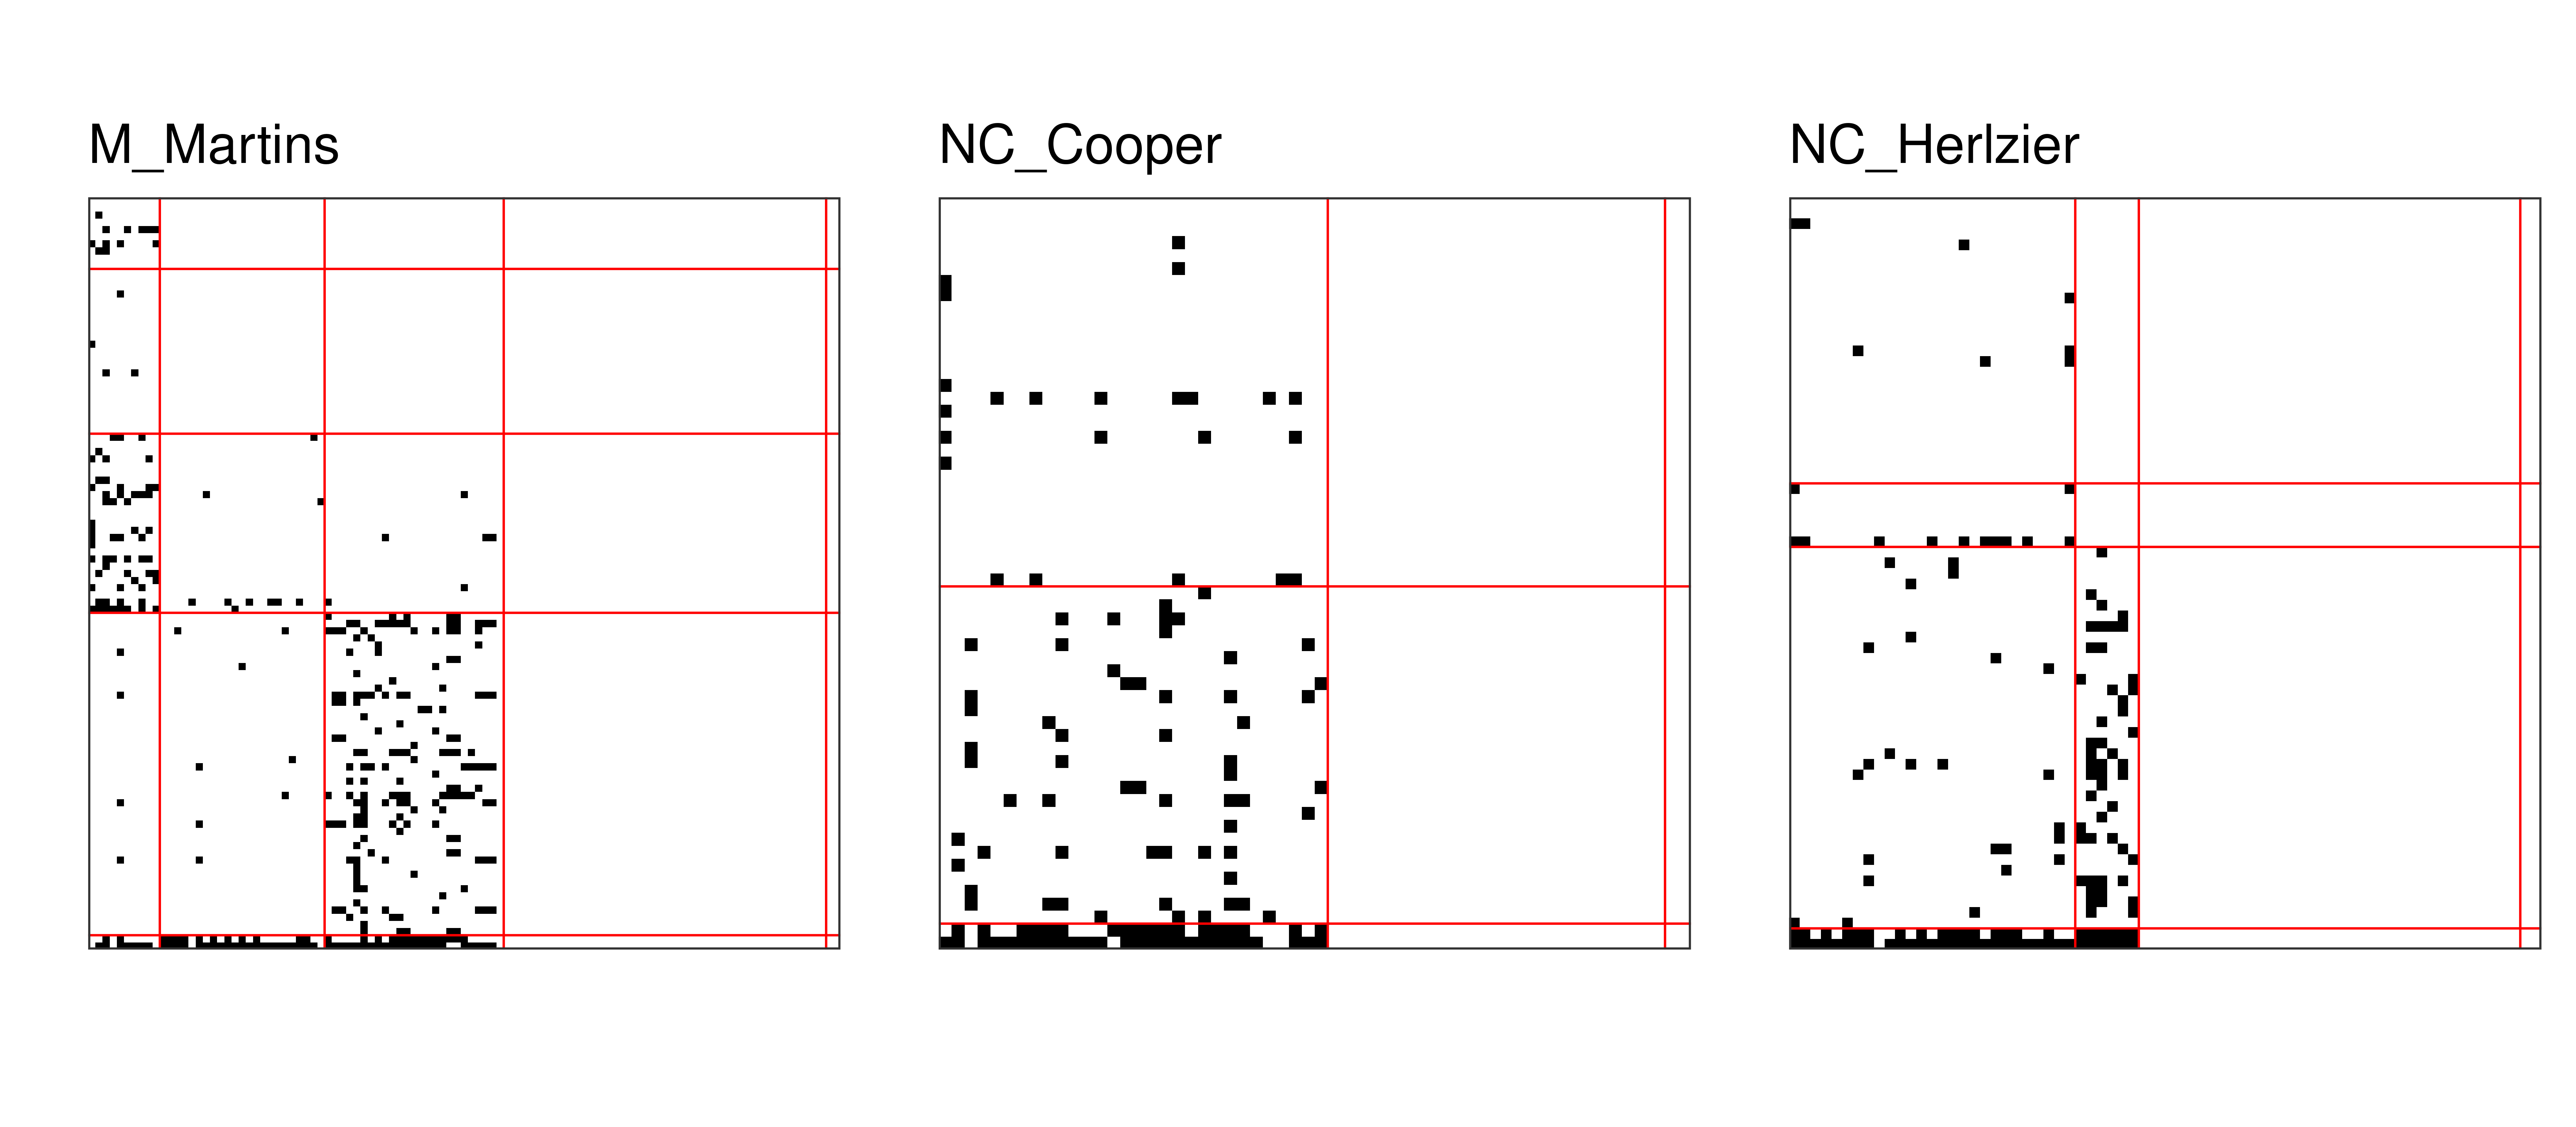
\includegraphics[width = .8\textwidth]{plots/plot_sbm_3net}}
   
Separate sbm
\end{frame}


%======================================================
\begin{frame}{Model choice}
%======================================================


\centering
\begin{tabular}{|c|c|}
\hline
Model & ICL \\
\hline
sepSBM & $-2080$\\
iid-colSBM& $-1966$ \\
$\pi$-colSBM &$-1982$ \\
$\dens$-colSBM & $-1969$\\
$\dens\pi$-colSBM&$-1989$ \\
\hline
\end{tabular}

\begin{itemize}
 \item Reject sepSBM : commun structure in the networks
\end{itemize}




\end{frame}




% %======================================================
% \begin{frame}{Our 4 consensus models}
% %======================================================
%   
% 
% \centering
% 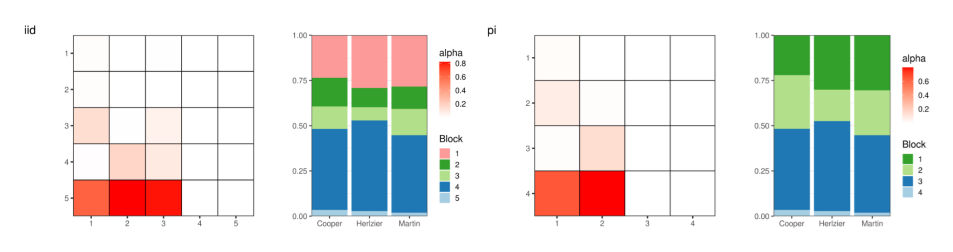
\includegraphics[width = \textwidth]{plots/plot_colsbm_3net_bis}
% \scriptsize{
% Left : iid ($-1966 $).  
% Right: $\picolSBM$ ($-1982$)
% %Bottom-left: $\denscolSBM$ ($-1969$). 
% %Bottom-right: 
% %$\denspicolSBM$ (-1989)
% }
% 
% \end{frame}

%======================================================
\begin{frame}{$\iidcolSBM$: the prefered model}
%======================================================
\centering
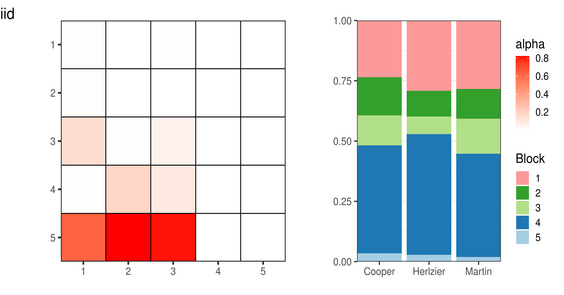
\includegraphics[width =0.5 \textwidth]{plots/plot_iidcolsbm}


\begin{itemize}
 \item Makes $5$ blocks
 \item  Block 3 (light green) is a small block
of intermediate trophic level species with some within block predation.

\item The higher trophic level is divided into 2 more blocks,
\begin{itemize}
\item block 2 (dark green) only preys on the 2 basal blocks
\item  block 1 (pink) preys on the intermediate block 3 level but only on the most connected basal species block.
\end{itemize}
\end{itemize}

\end{frame}


%======================================================
\begin{frame}{$\picolSBM$}
%======================================================
\centering
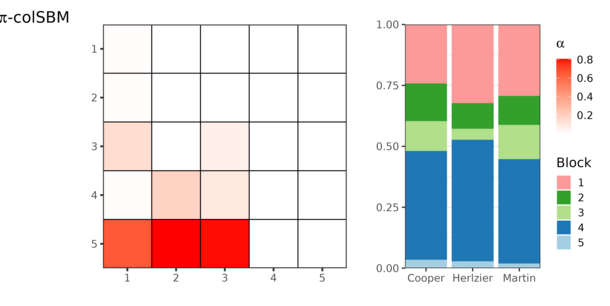
\includegraphics[width =0.5 \textwidth]{plots/plot_picolsbm}

\begin{itemize}
\item Also 5 blocks.
\item There are no empty blocks 
\item the block
proportions are roughly corresponding to the ones of iid-colSBM . 
\item Flexibility of the $\picolSBM$ of little use compared to the iid-colSBM
on this collection.
\end{itemize}

\end{frame}

%======================================================
\begin{frame}{Conclusion}
%======================================================
\begin{itemize}
 \item The three networks do share a commun structure. 
\item We can identify the species playing the same role across networks (ecosytems)
\item Other results
\begin{itemize}
\item Quality of prediction when missing data. 
\item Application in sociology: advices between lawyers, researchers  or priests
\item Clustering of networks. Application on a database of 80 networks. 
\end{itemize}


 
\end{itemize}


\end{frame}

 
%======================================================
\begin{frame}{Work in progress}
%======================================================
\begin{itemize}
\item Develop a wide variety of models
\item Very active research field in our group
\item Various extensions in progress
\begin{itemize}
\item Taking into account the incertitude of reconstruction of the networks (data from metagenomics)
\item Extension to large multilayer networks such as interactome
\item Looking for tools to compare networks : plant health submitted to combination of stress
\end{itemize}
\end{itemize}

\end{frame}





%====================================================================

\begin{frame}[allowframebreaks]{References}
%====================================================================


  \bibliography{biblio}
  \bibliographystyle{apalike}

\end{frame}

\section*{Partition of networks according to their  mesoscale structure}

%======================================================
\begin{frame}{To go further : partitionning a collection of networks}
%======================================================
  
\begin{itemize}
 \item If the networks in a collection do not have the same connectivity structure, we aim to partition them accordingly.
 \item Finding   a partition $\mathcal{G} = (\Mcal_g)_{g  = 1, \dots,G}$ of $\{1, \dots,M\}$. %, such that  $\cup_{g} \mathcal{M}_g = \{1, \dots, M\}$.  
 
 such that
 
\begin{equation*}
 \forall g \in \{1, \dots, G\}, \quad \forall m \in \Mcal_g, \quad  \Xm \sim \SBM(K^g, \bpim, \balpha^g)
\end{equation*}

networks belonging to the subcollection $\Mcal_g$ share the same mesoscale structure given by  $\picolSBM$. % structure.  
 \end{itemize}

 \end{frame}
 
%======================================================
\begin{frame}{Scoring a partition}
%======================================================

\begin{itemize}
\item To any partition $\mathcal{G}$ we associate the following score: 
\begin{equation*}\label{coll:ICL:partition}
  \Sc(\Gcal) =   \sum_{g  = 1} ^G \BICL((\Xm)_{m \in \Mcal_g}, \widehat{K^g}).
\end{equation*}

\item Best partition $\Gcal$ is chosen as follows:  
\begin{equation*}
    \Gcal^* = \argmax_{\Gcal} \Sc(\Gcal).
\end{equation*}


\end{itemize}
  
\end{frame}  
    

%======================================================
\begin{frame}{Partition of the networks from the Mangal database}
%======================================================

\begin{itemize}
 \item $67$ networks issued from the \href{https://mangal.io}{Mangal database} belonging to 33 datasets.
\cite{rmangal}

\item predation networks which are all directed networks with more than $30$ species,
\item number of species ranges from $31$ to $106$ ($3395$ in total) by network
\item Density ranging from $.01$ to $.32$ ($14934$ total predation links). 
\end{itemize}


\alert{Aim} use our model to propose partition of the networks into group of networks with common mesoscale structure.  

\end{frame}


%======================================================
\begin{frame}{Partition on the networks from the Mangal database}
%======================================================



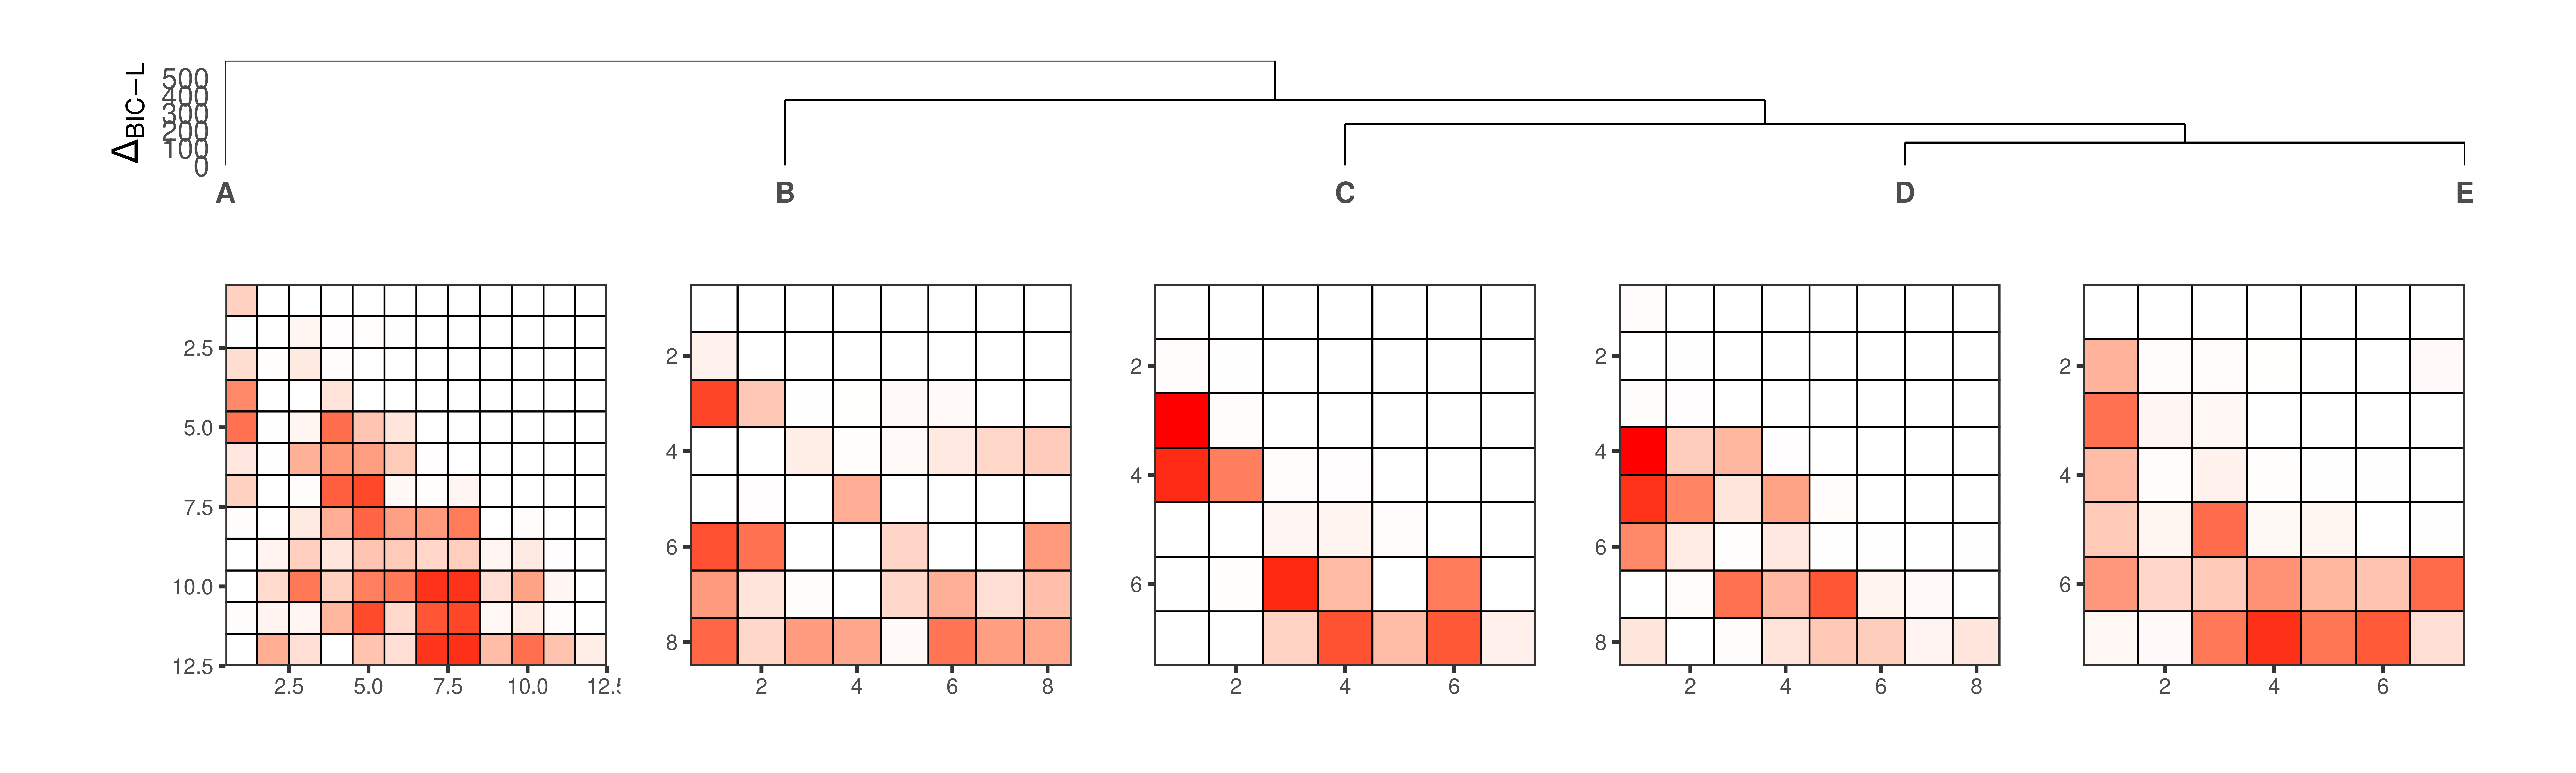
\includegraphics[width=\hsize]{plots/rmangal_pi_newpen_dend_meso}

\end{frame}
%======================================================
\begin{frame}{Partition on the networks from the Mangal database}
%======================================================


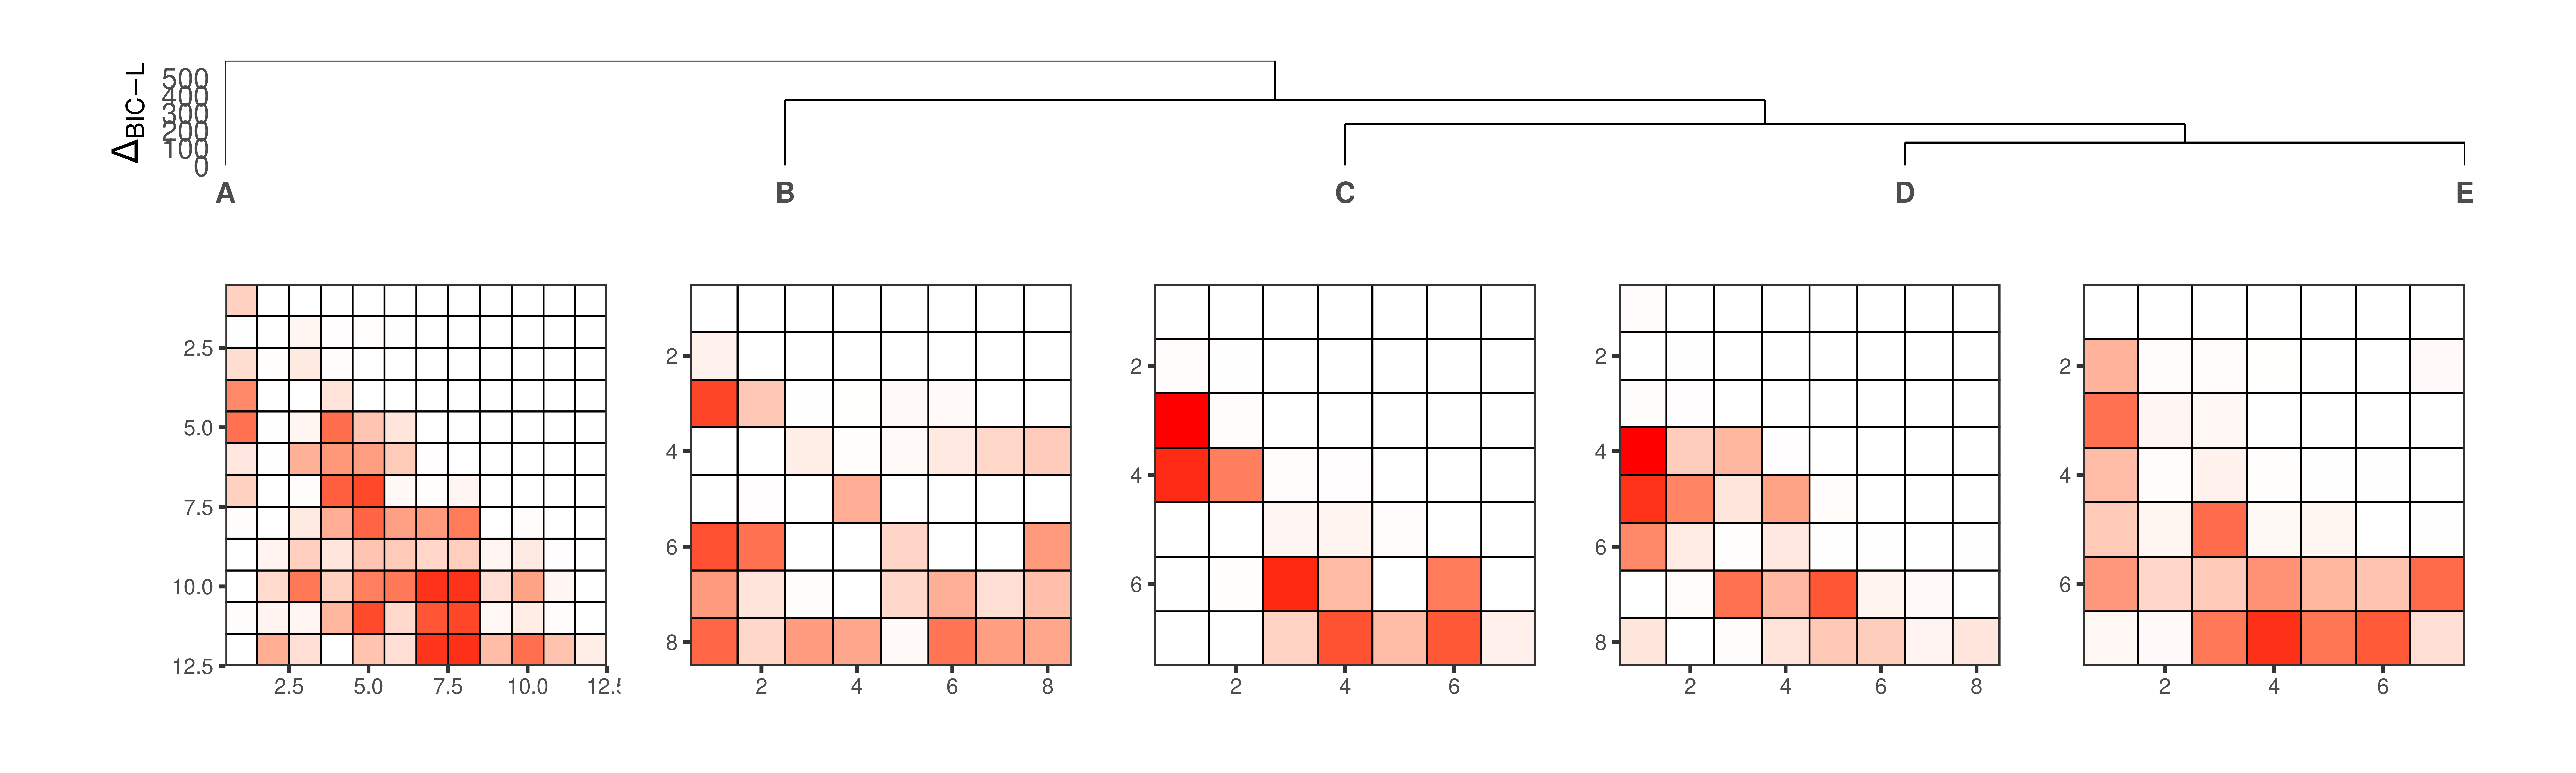
\includegraphics[width=\hsize]{plots/rmangal_pi_newpen_dend_meso}

     
 \alert{Groupe A} 
 \begin{itemize}
  \item $7$ networks and $12$ blocks are required to describe this group of networks
  \item $5$ networks are issued from the same dataset (id: 80).
  \item These $5$ networks populate the $12$ blocks, while the other $2$ networks only populate parts of them.
  \item Average density is about $0.18$
  \item Blocks $1$ to $3$ represent the higher trophic levels, blocks $4$ to $8$ the intermediate ones and block $9$ to $12$ the lower ones.    
 \end{itemize}
 


\end{frame}


%======================================================
\begin{frame}{Partition on the networks from the Mangal database}
%======================================================

    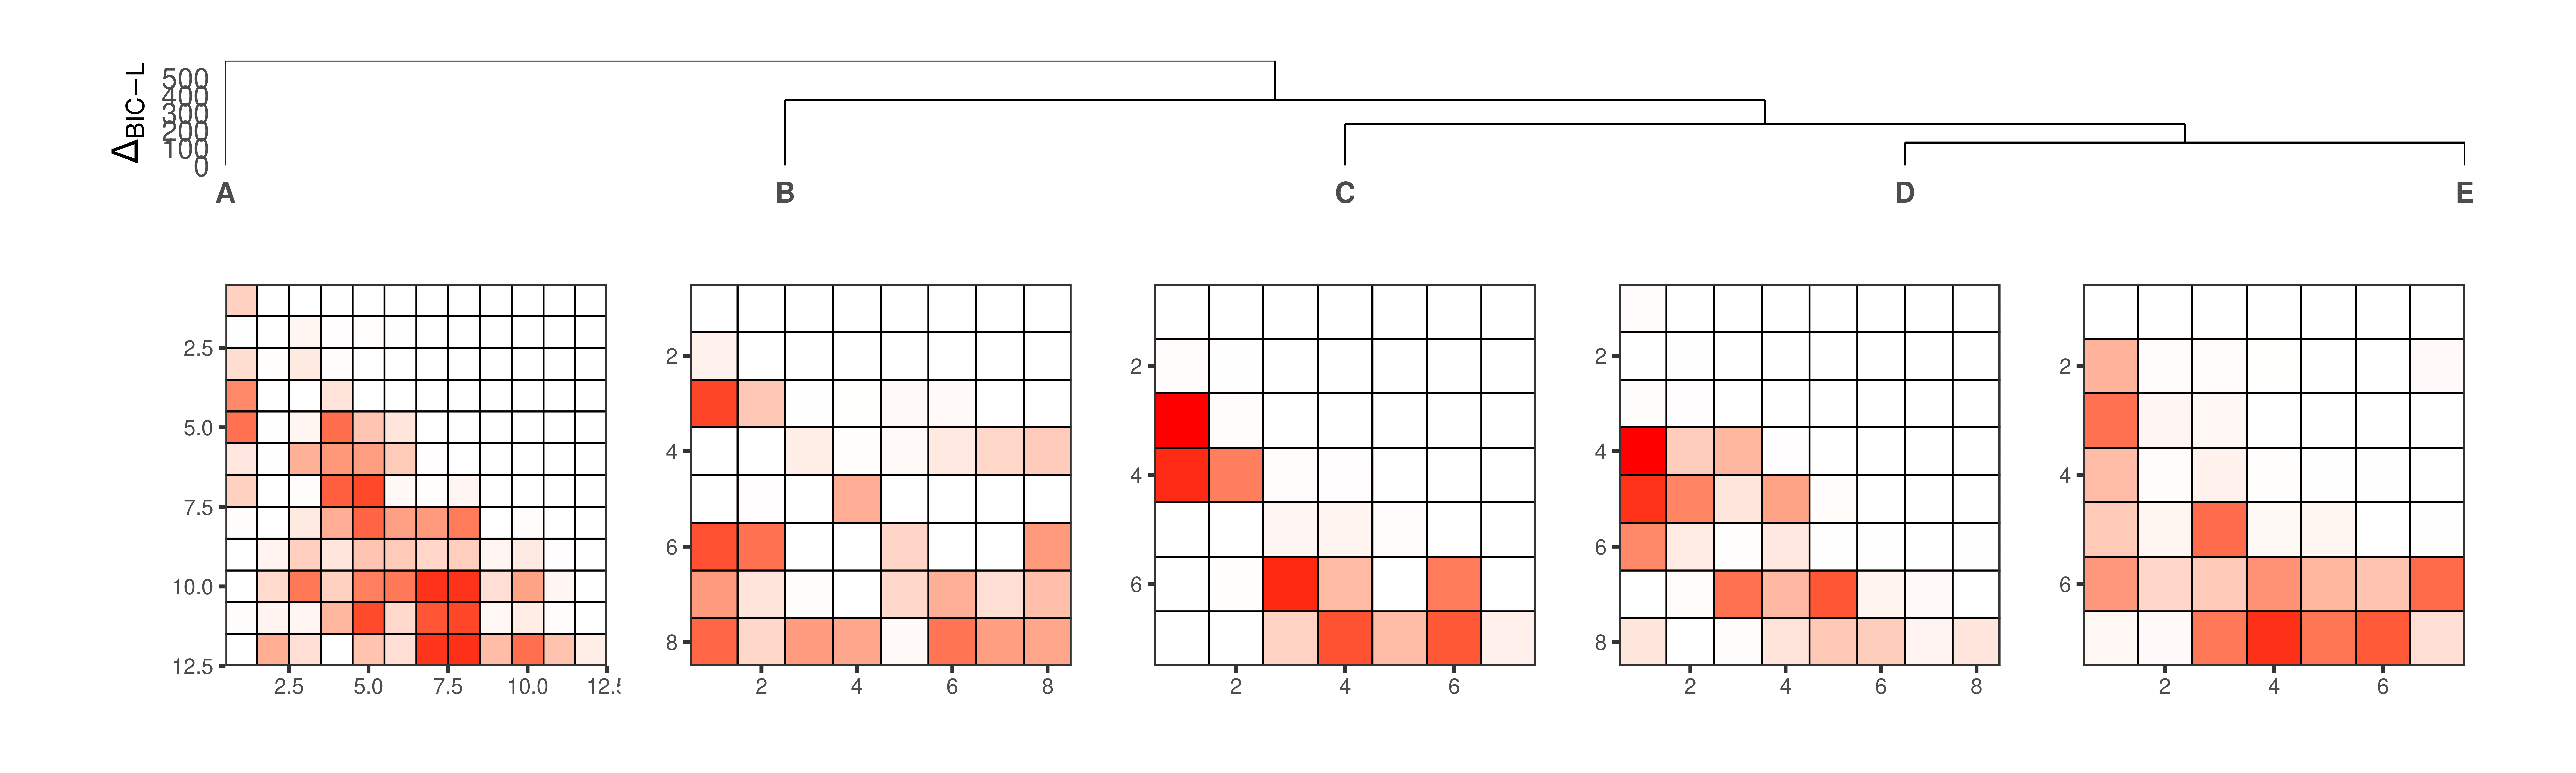
\includegraphics[width=\hsize]{plots/rmangal_pi_newpen_dend_meso}
     

\alert{Group B} : structure with 8 blocks 
\begin{itemize}
 \item $26$ networks with heterogeneous size and density. 
 \item Issued from various datasets
 \item Most networks populate only parts of the $8$ blocks
 \item Block $4$ is represented in only $5$ networks where it is either an intermediate or a bottom trophic level.  
 %\item It introduces some symmetry in the connectivity matrix rendering it difficult to order the blocks by trophic order. 
 \item Species from top trophic levels prey on basal species.  
\end{itemize}

\end{frame}


%======================================================
\begin{frame}{Partition on the networks from the Mangal database}
%======================================================

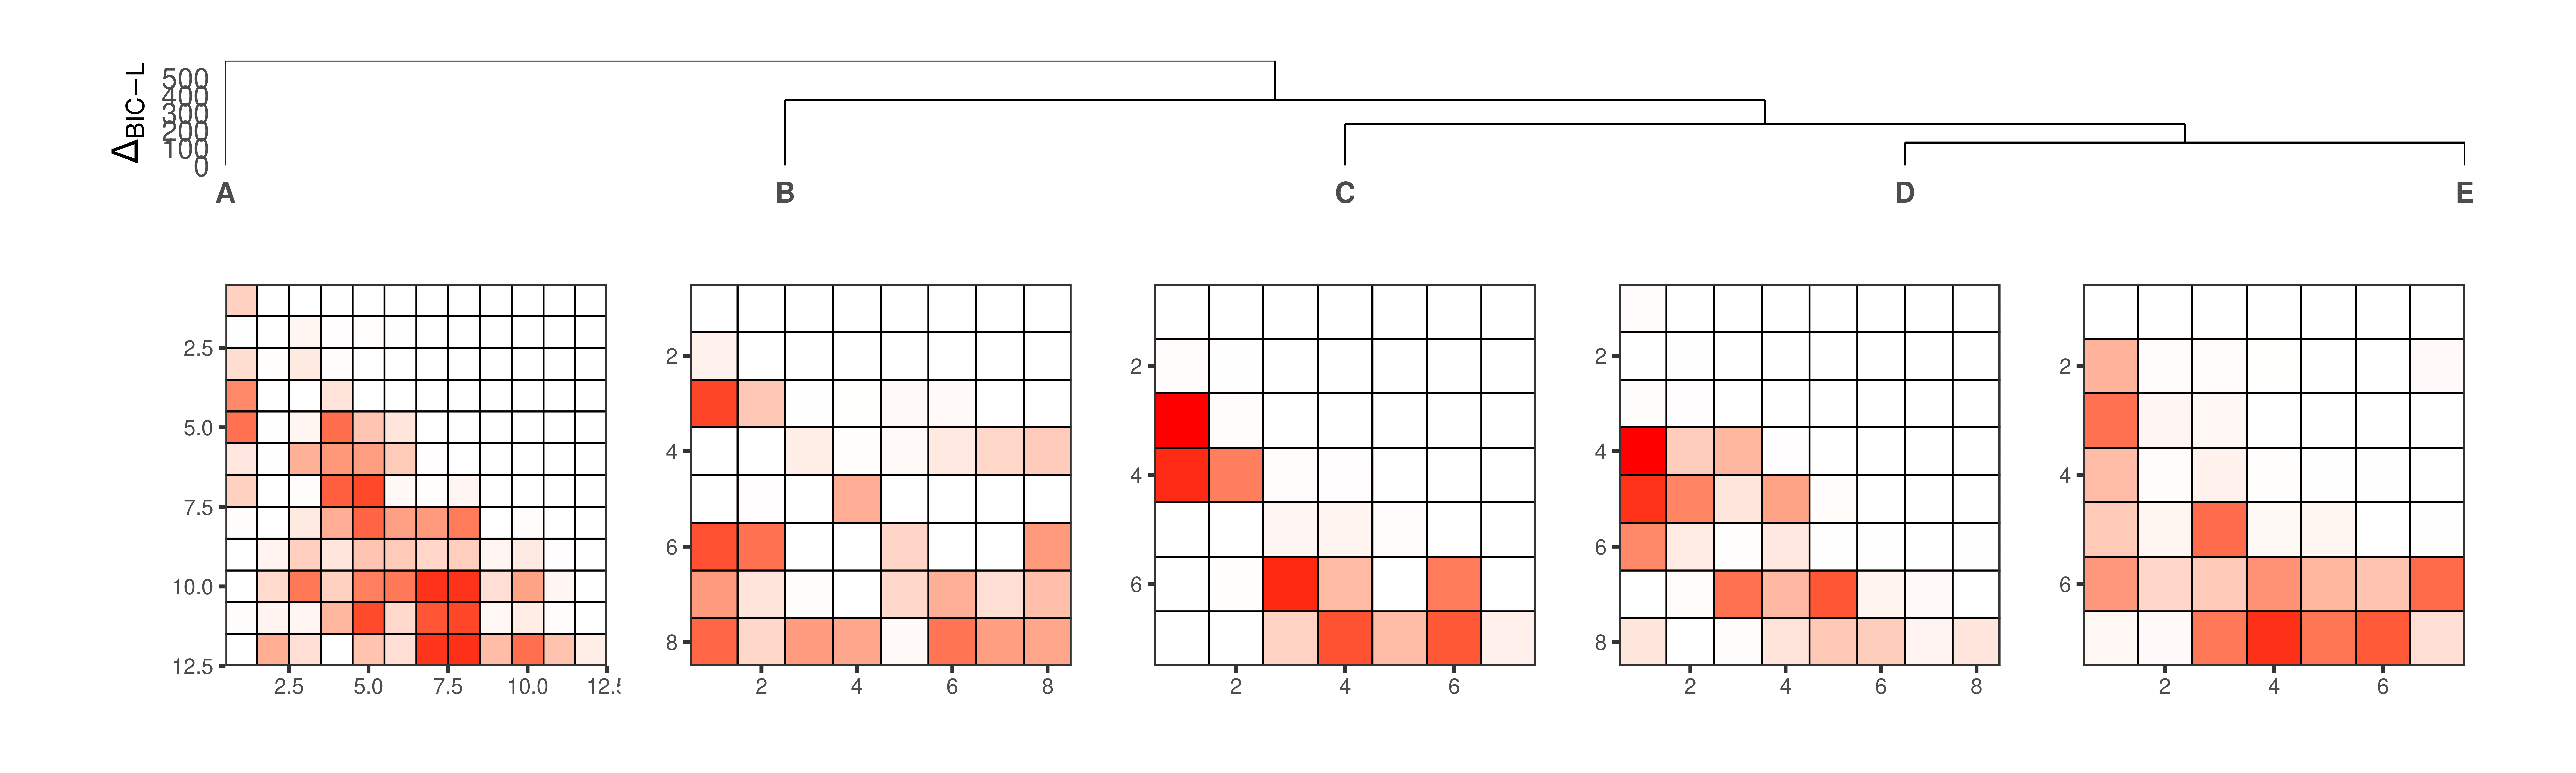
\includegraphics[width=\hsize]{plots/rmangal_pi_newpen_dend_meso}
    

\alert{Group C} : structure with 7 blocks 
\begin{itemize}
 \item $6$ networks with density ranging from $.06$ to $.11$. 
 \item All networks are represented in $5$ or $6$ of the $7$ blocks, including the first three blocks. 
 \item  $3$ of the $5$ networks of dataset $48$ (diff. collecting sites). 
 \item Top trophic level divided into $2$ blocks, species from those blocks preying only on intermediate trophic level species. 
 
%  \begin{itemize}
%  \item Species from block $2$ prey on  species from block $4$, which prey more on basal species (block $7$) than on others intermediate trophic species (block $6$), 
%  \item Species from block $1$ prey on species from block $3$ and $4$, block $3$ exhibiting the inverse behavior of block $4$.  
% \end{itemize}
\end{itemize}

\end{frame}

%======================================================
\begin{frame}{Partition on the networks from the Mangal database}
%======================================================

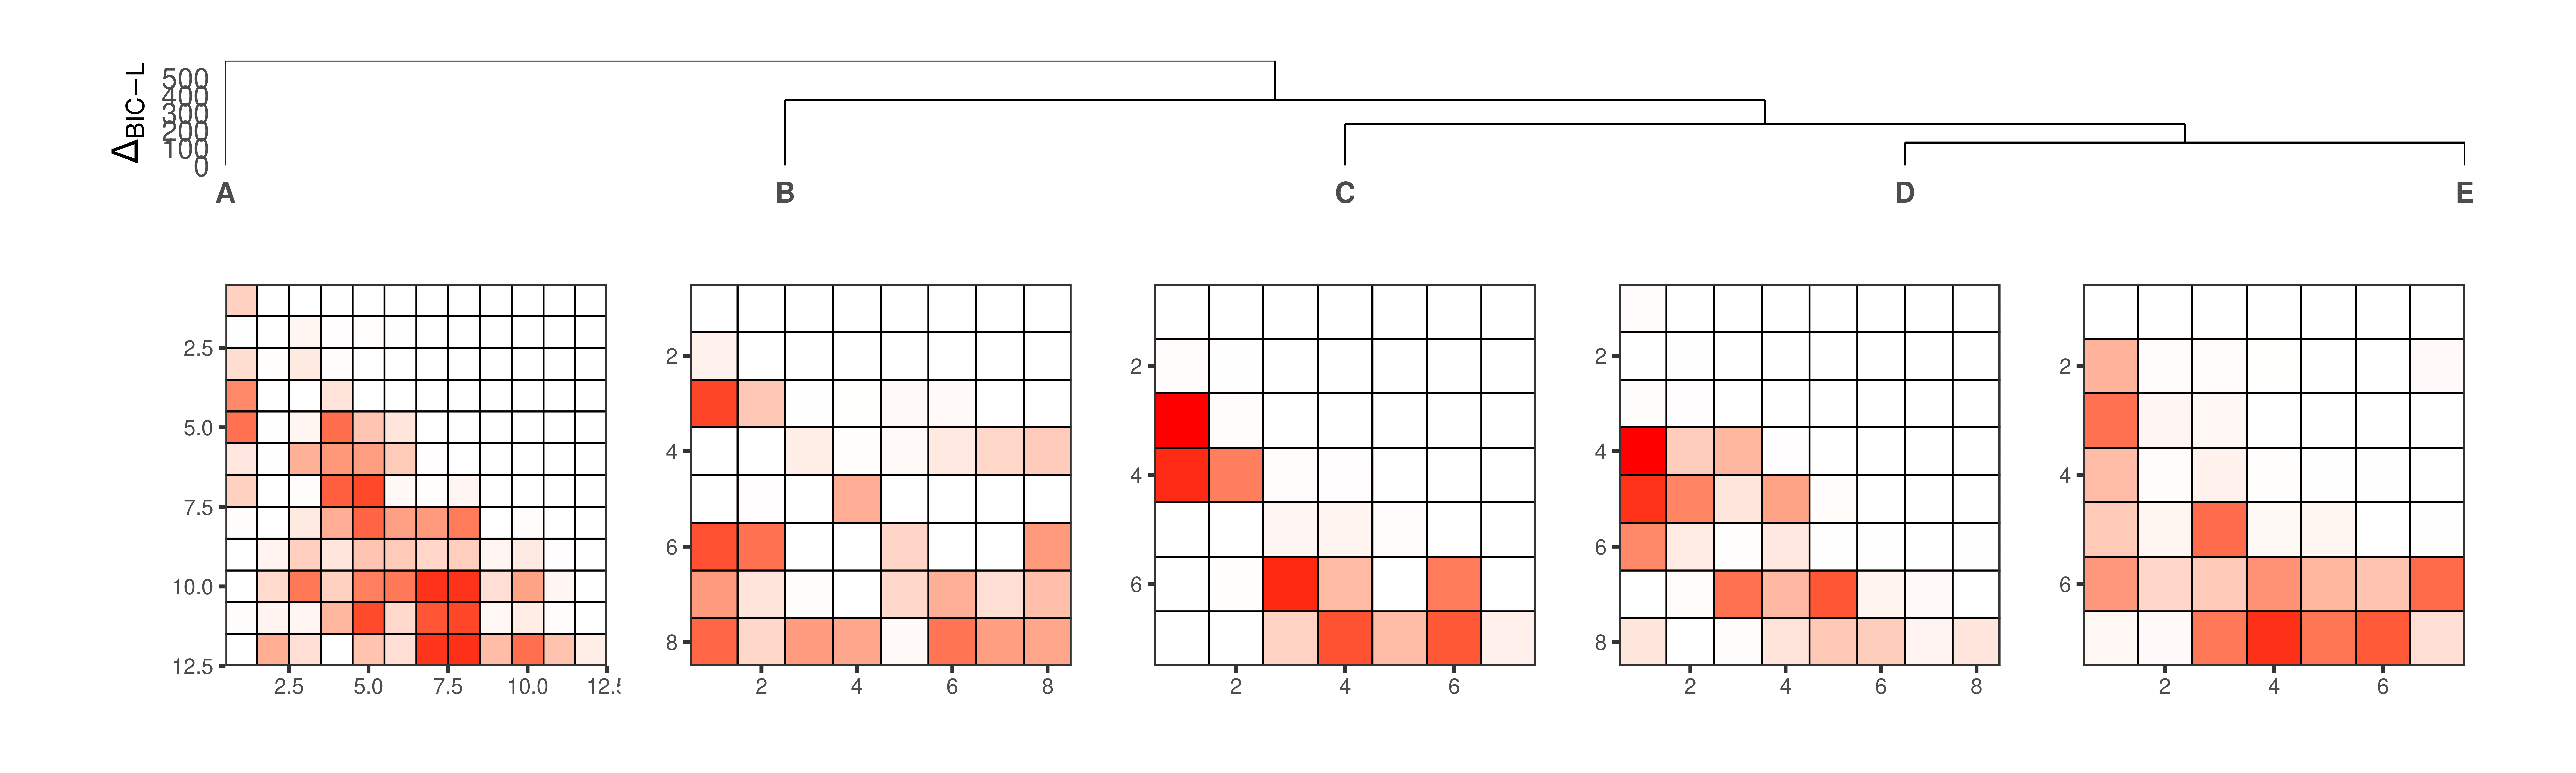
\includegraphics[width=\hsize]{plots/rmangal_pi_newpen_dend_meso}
    

\alert{Group D} : structure with 7 blocks 
\begin{itemize}
 \item  $23$ networks. 
 \item The $10$ networks from dataset $157$ (stream food webs from New Zealand) are divided between groups \textbf{B} and \textbf{D} based on the type of ecosystem. 
 The data from group \textbf{B} were collected in creeks, while the one from group \textbf{D} were collected on streams. 
\end{itemize}
\end{frame}


%======================================================
\begin{frame}{Partition on the networks from the Mangal database}
%======================================================

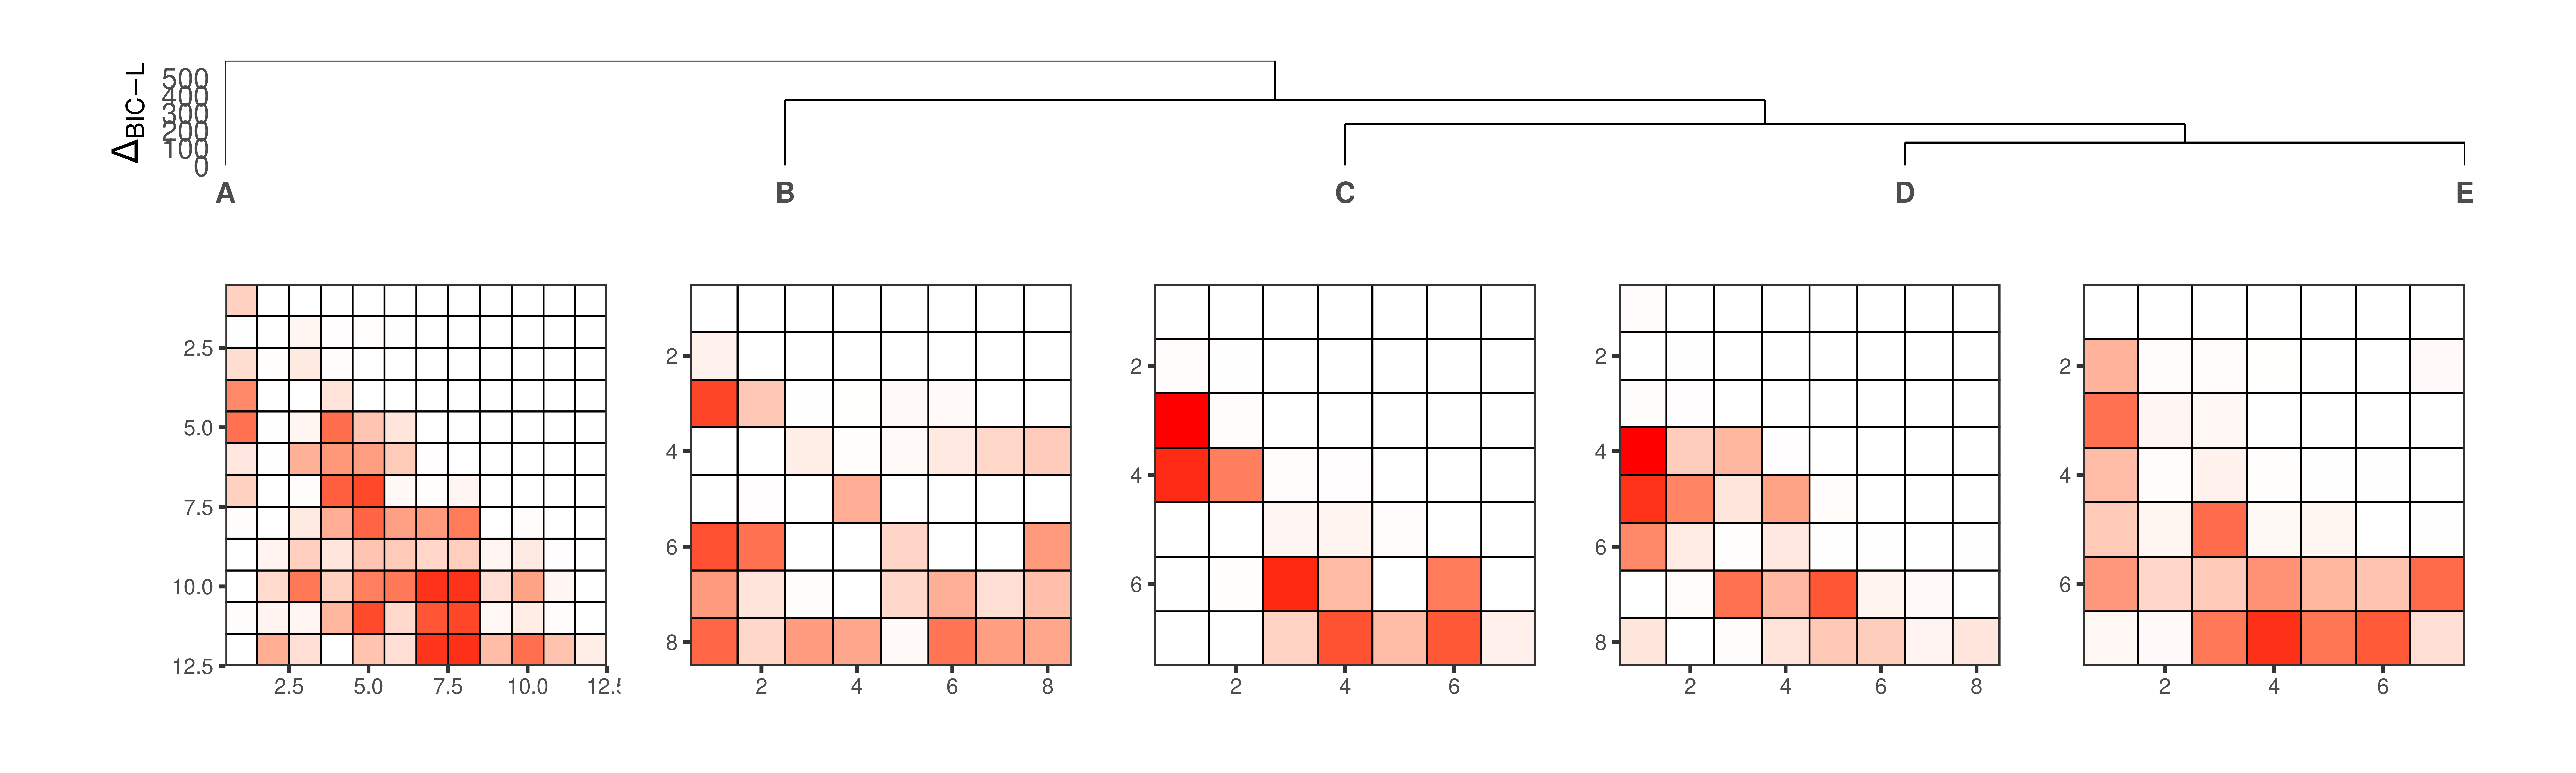
\includegraphics[width=\hsize]{plots/rmangal_pi_newpen_dend_meso}
   
\alert{Group E} : structure with 7 blocks 

   
\end{frame}

% 
% 
% %====================================================================
%  \begin{frame}{Comments on the   ICL versus BIC}\label{BIC-ICL}
% % %====================================================================
% \begin{block}{Conjecture}
% \begin{eqnarray*}
%  BIC(\M)  &=&  \log \ell(\Xall; \hat{\theta}, \M) - \pen(\M)
% \end{eqnarray*}
% with the same penalty
%  \end{block}
% 
% \begin{itemize}
% \item Under this conjecture
% \begin{eqnarray*}
%  ICL(\M)  &= & BIC(\M)  +   \sum_{\Zall} p(\bZ | \Xall;\hat \theta_{K}) \log p(\bZ | \Xall; \hat \theta_{K})\\
%  &=& BIC(\M)  -   \mathcal{H}( p(\cdot | \Xall;\hat \theta_K)) 
% \end{eqnarray*}
% \item As a consequence, because of the entropy,  ICL  will encourage clustering with well-separated groups 
% \item 
% $$ 
%  \widehat{ICL}(\mathcal{M})  =BIC(\mathcal{M})  +   \sum_{\Zall} \mathcal{R}_{\Xall}(\bZ,\widehat{\btau})  \log \mathcal{R}_{\Xall,\widehat{\btau}}({\bZ}) -  \mathbf{KL}[\mathcal{R}_{\Xall,\widehat{\btau}}, p(\cdot | \Xall;\widehat{\theta})]\,. 
% $$
% 
% \end{itemize}
% 
%  
% \hyperlink{ICL}{\beamergotobutton{Back to the presentation}}
%  \end{frame}
%  
 

% 
% %====================================================================
% \begin{frame}{About bipartite networks}\label{bipartite}
% %==================================================================== 
% \begin{itemize}
%  \item Example : plant / pollinators
%   \item Bi-clustering
%   \item Same principle
% 
%  
% \begin{itemize}
% \item $K_1$ blocks of plants, $K_2$ blocks of pollinators
% \item 2 sets of latent clustering variables $(Z^{plant}_i)_{i=1,\dots,n_1},(Z^{poll}_j)_{j=1,\dots,n_2}$...
% \item Conditionnally to latent variables: 
% $(Y_{ij})$ independent and 
% \begin{eqnarray*}
%  Y_{ij}  | Z^{plant}_i=k, Z^{poll}_j=\ell \sim  \mathcal{B}ern(\alpha_{k\ell})  
% \end{eqnarray*}
% \end{itemize}
% \end{itemize}
% \end{frame}

% %====================================================================
% \begin{frame}{About multipartite networks}\label{multipartite}
% %==================================================================== 
% 
% \begin{itemize}
%  \item Involving more than two functional groups  ($Q$)
%  \item For instance plants: pollinators, seed-dipersal birds, ants...  
%  \begin{itemize}
%  \item $Q$-clustering : $Q$ sets of latent clustering variables $(Z^{q}_i)_{i=1,\dots,n_q}$...
% \item $K_q$ blocks in each functional group
% \item Conditionnally to latent variables: 
% $(Y^{qq'}_{ij})$ independent and 
% \begin{eqnarray*}
%  Y^{qq'}_{ij}  | Z^{q}_i=k, Z^{q'}_j=\ell \sim  \mathcal{B}ern(\alpha^{qq'}_{k\ell})  
% \end{eqnarray*}
% \end{itemize}
% \item Inference, model selection procedure : adapted
% \item Package \textsf{sbm}
% \end{itemize}
% \end{frame}



\end{document}
